\documentclass[12pt, titlepage]{article}

\usepackage{booktabs}
\usepackage{tabularx}
\usepackage{hyperref}
\usepackage{comment}
\usepackage{enumitem}
\usepackage[margin=1in]{geometry}
\usepackage{amsmath}
\usepackage{amsthm}
\usepackage{amssymb}
\usepackage{graphicx}
\usepackage{multirow}
\usepackage{subcaption}

\hypersetup{
    colorlinks,
    citecolor=blue,
    filecolor=black,
    linkcolor=red,
    urlcolor=blue
}

\newcommand{\progname}{Realm}
\newcommand{\authname}{Team \#13, ARC
    \\ Avanish Ahluwalia
    \\ Russell Davidson
    \\ Rafey Malik
    \\ Abdul Zulfiqar}

\usepackage{hyperref}
    \hypersetup{colorlinks=true, linkcolor=blue, citecolor=blue, filecolor=blue,
                urlcolor=blue, unicode=false}
    \urlstyle{same}

\begin{document}

\title{User Manual for \\ \progname{}: An AR Tours App}
\author{\authname}
\date{April 4, 2025}

\maketitle

\pagenumbering{roman}

\newpage

\tableofcontents

\newpage

\pagenumbering{arabic}

%-----------------------------
\section{Introduction}
\subsection{Purpose of the Manual}
The purpose of this user manual is to provide comprehensive instructions for using \progname{} effectively. It is designed to assist users in understanding the app's features, functionalities, and troubleshooting common issues.

\subsection{Scope}
The user manual covers the installation process, account setup, user interface overview, features and functionalities, task-based procedures, troubleshooting, accessibility features, and additional resources.

\subsection{Audience}
The manual is intended for all users of \progname{}, including beginners who are new to the app and advanced users looking for detailed instructions on specific features. It is useful for both \textbf{General} users and \textbf{Organizational} users. The manual is also useful for administrators who may need assistance with installation, app configuration and troubleshooting.

%-----------------------------
\section{Getting Started}
\subsection{System Requirements}
To run \textbf{\progname{}}, user devices must meet the following minimum requirements:
\begin{itemize}[leftmargin=*]
    \item \textbf{Operating System:} Android 8.0 (Oreo) or later, iOS 12.0 or later
    \item \textbf{RAM:} Minimum 4 GB
    \item \textbf{Storage:} At least 200 MB of free space
    \item \textbf{Internet Connection:} Required for downloading the app and accessing online features
    \item \textbf{Camera:} Required for AR object projections
    \item \textbf{GPS and Location Services:} Required to detect the user's location relative to active Tours and their corresponding AR objects.
    \item \textbf{System Permissions:} The app requires access to the camera, location services and read/write to storage.
\end{itemize}

\subsection{Installation Instructions}
Since \textbf{\progname} is a mobile application that cannot be uploaded to Apple App Store and Google Play Store due to inability to meet their publishing requirements, the app must be built in Unity and installed on the device using the following steps:
\begin{itemize}[leftmargin=*]
    \item \textbf{Download the Source Code:} Download the source code from the GitHub repository \href{https://github.com/russellrd/realm}{here}.
    \item \textbf{Install Unity:} Ensure you have Unity installed on your computer. You can download it from the official Unity website.
    \item \textbf{Open the Project:} Open Unity and load the downloaded project.
    \item \textbf{Build Settings:} Go to \texttt{File $>$ Build Settings}, select the target platform (iOS or Android), and click on "Switch Platform".
    \item \textbf{Build the Project:} Once the platform has been switched, click on the "Build and Run" button. This will compile the project and create an APK (for Android) or an Xcode project (for iOS).
    \item \textbf{Connect Device:} Connect your mobile device to your computer via USB.
    \item \textbf{Install on Device:} Follow the instructions for your platform to install the app on your device.
          \begin{itemize}[leftmargin=*]
              \item \textbf{For Android:} Enable USB debugging on your device and use ADB to install the APK.
              \item \textbf{For iOS:} Use Xcode to deploy the app to your device.
          \end{itemize}
    \item \textbf{Launch the App:} Once installed, find the app icon on your device's app menu and tap to launch it.
    \item \textbf{Permissions:} Upon first time launching the app, you will be prompted to grant permissions for camera and location access. Accept these permissions to use the app's features.
\end{itemize}

\textbf{Note:} Additional installation instructions can be found in the \href{https://github.com/russellrd/realm/blob/main/INSTALL.md}{INSTALL.md} file in the project repository.

\subsection{Account Setup}
When the user opens the app for the first time, they will need to create an account. The user will be prompted to enter their email address and password. \hyperref[fig:setup1]{Instead}, they should press ``Register'' to create a new account. \\
Then, the user must enter their username, email address and password. After that, user will also be asked to select their user type, either \textbf{General} or \textbf{Organizational}. The \hyperref[fig:setup1]{visuals below} show the process of creating an Organizational user account and logging in (For \emph{General} users, they select \texttt{General} in the first dropdown).

\begin{figure}[ht!]
    \centering
    \begin{subfigure}[b]{0.48\textwidth}
        \centering
        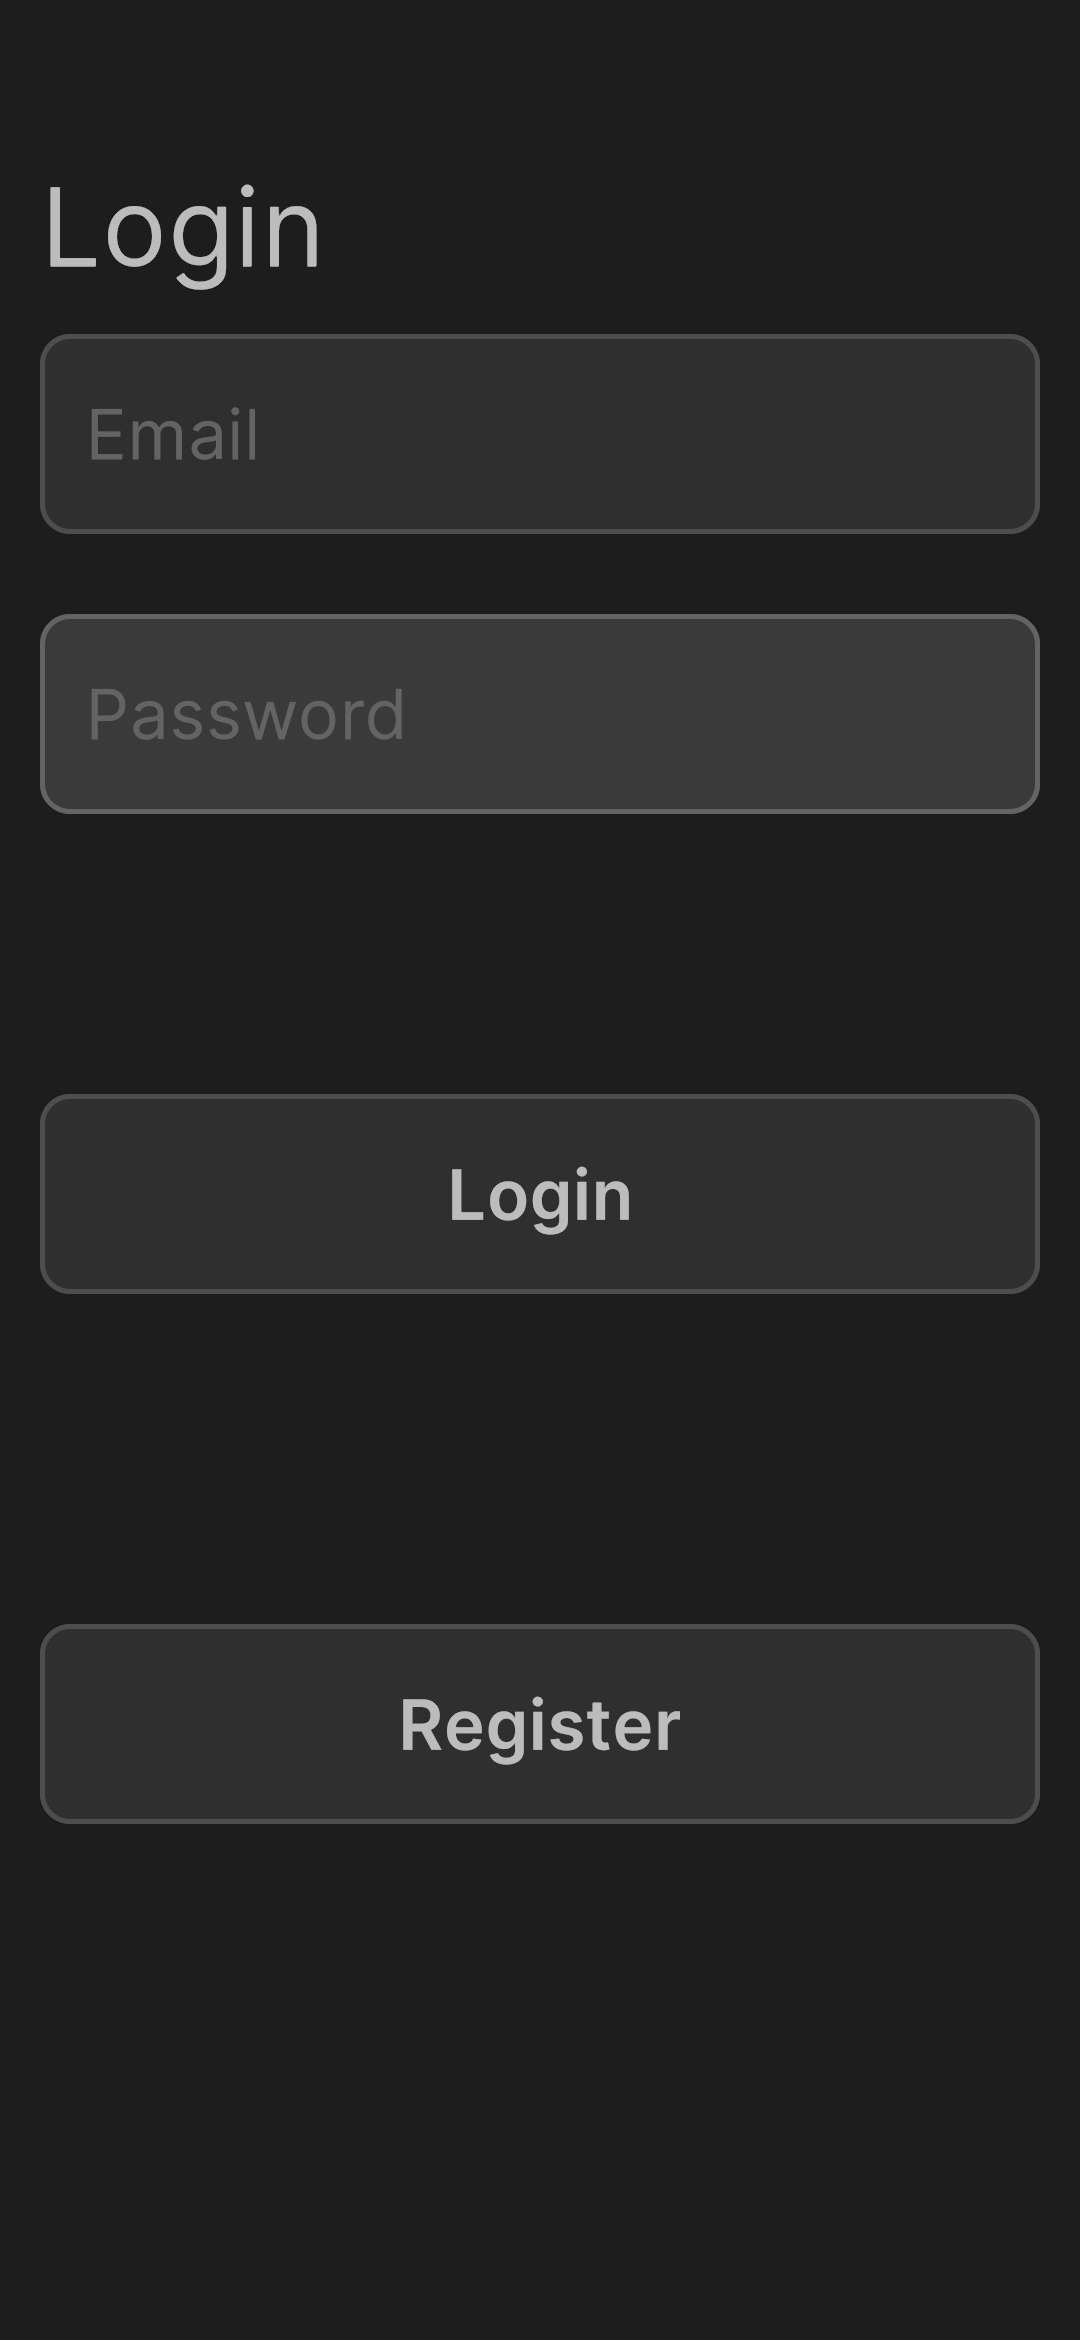
\includegraphics[width=\textwidth]{login1.png}
    \end{subfigure}
    \hfill
    \begin{subfigure}[b]{0.48\textwidth}
        \centering
        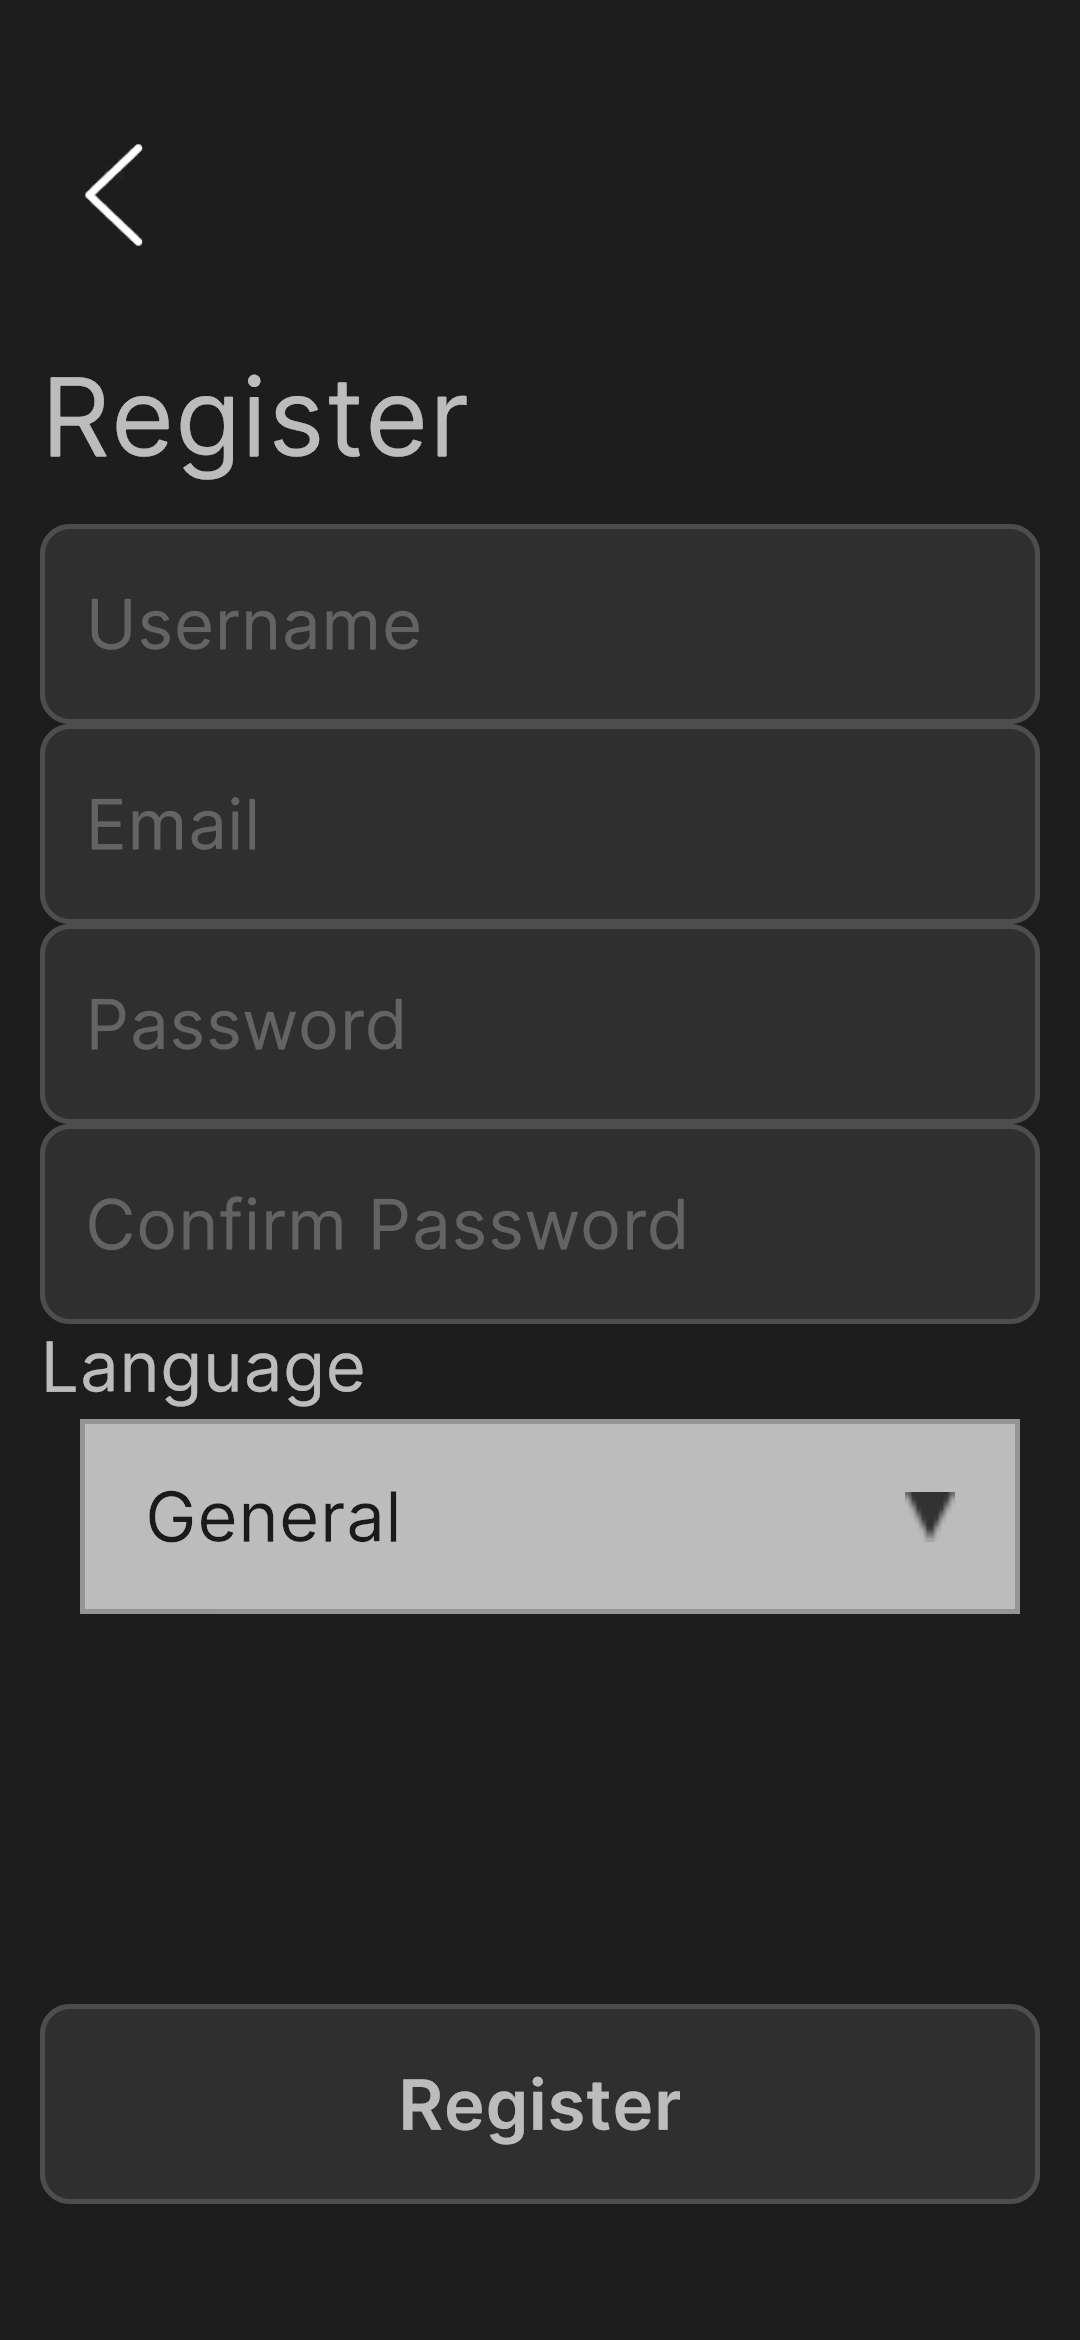
\includegraphics[width=\textwidth]{register1.png}
    \end{subfigure}
    \caption{Navigating to Account Creation}
    \label{fig:setup1}
\end{figure}

\newpage
\begin{figure}[ht!]
    \centering
    \begin{subfigure}[b]{0.48\textwidth}
        \centering
        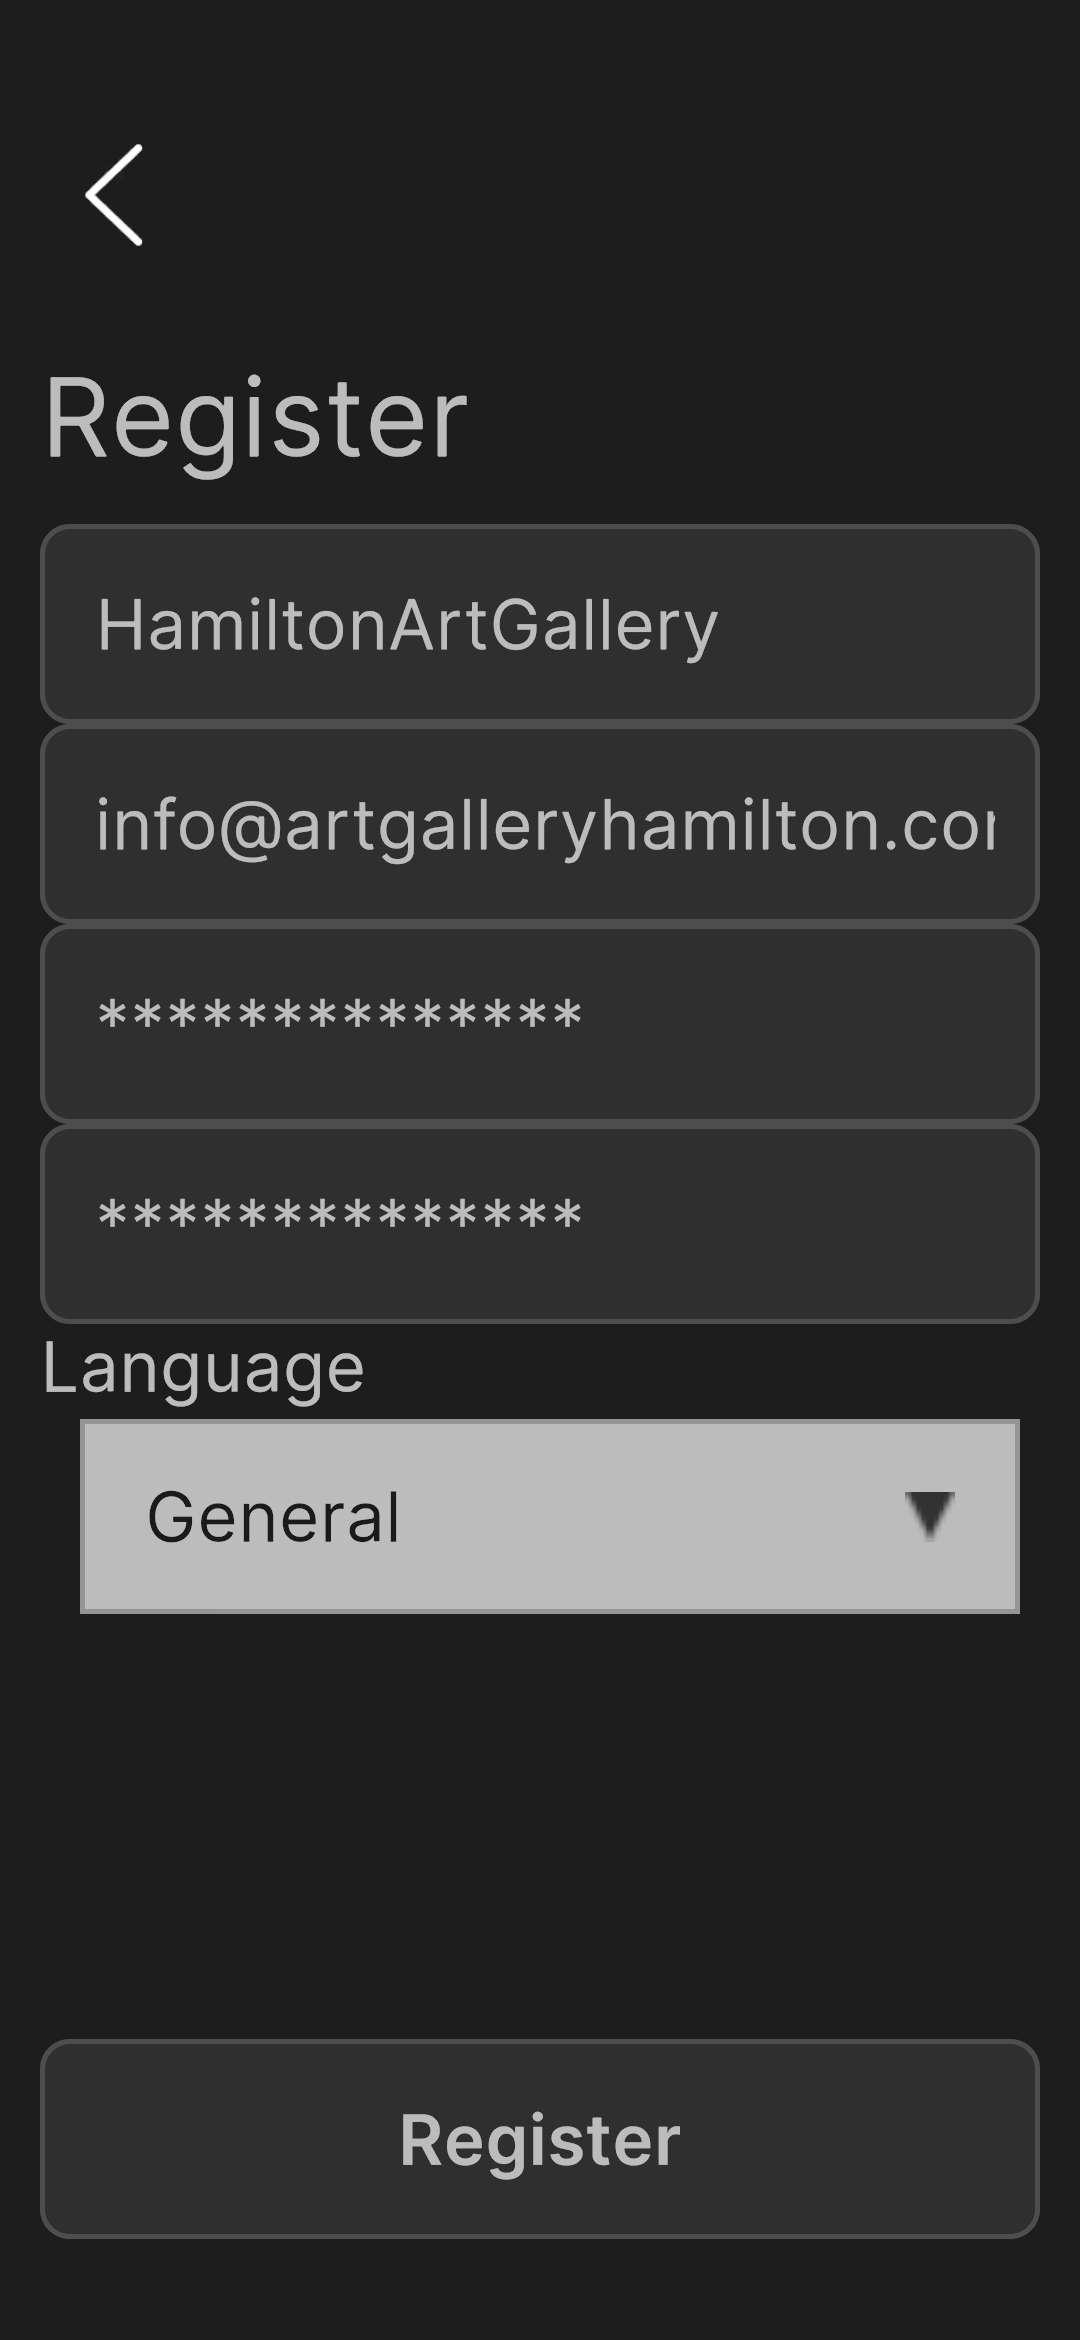
\includegraphics[width=\textwidth]{register2.png}
    \end{subfigure}
    \hfill
    \begin{subfigure}[b]{0.48\textwidth}
        \centering
        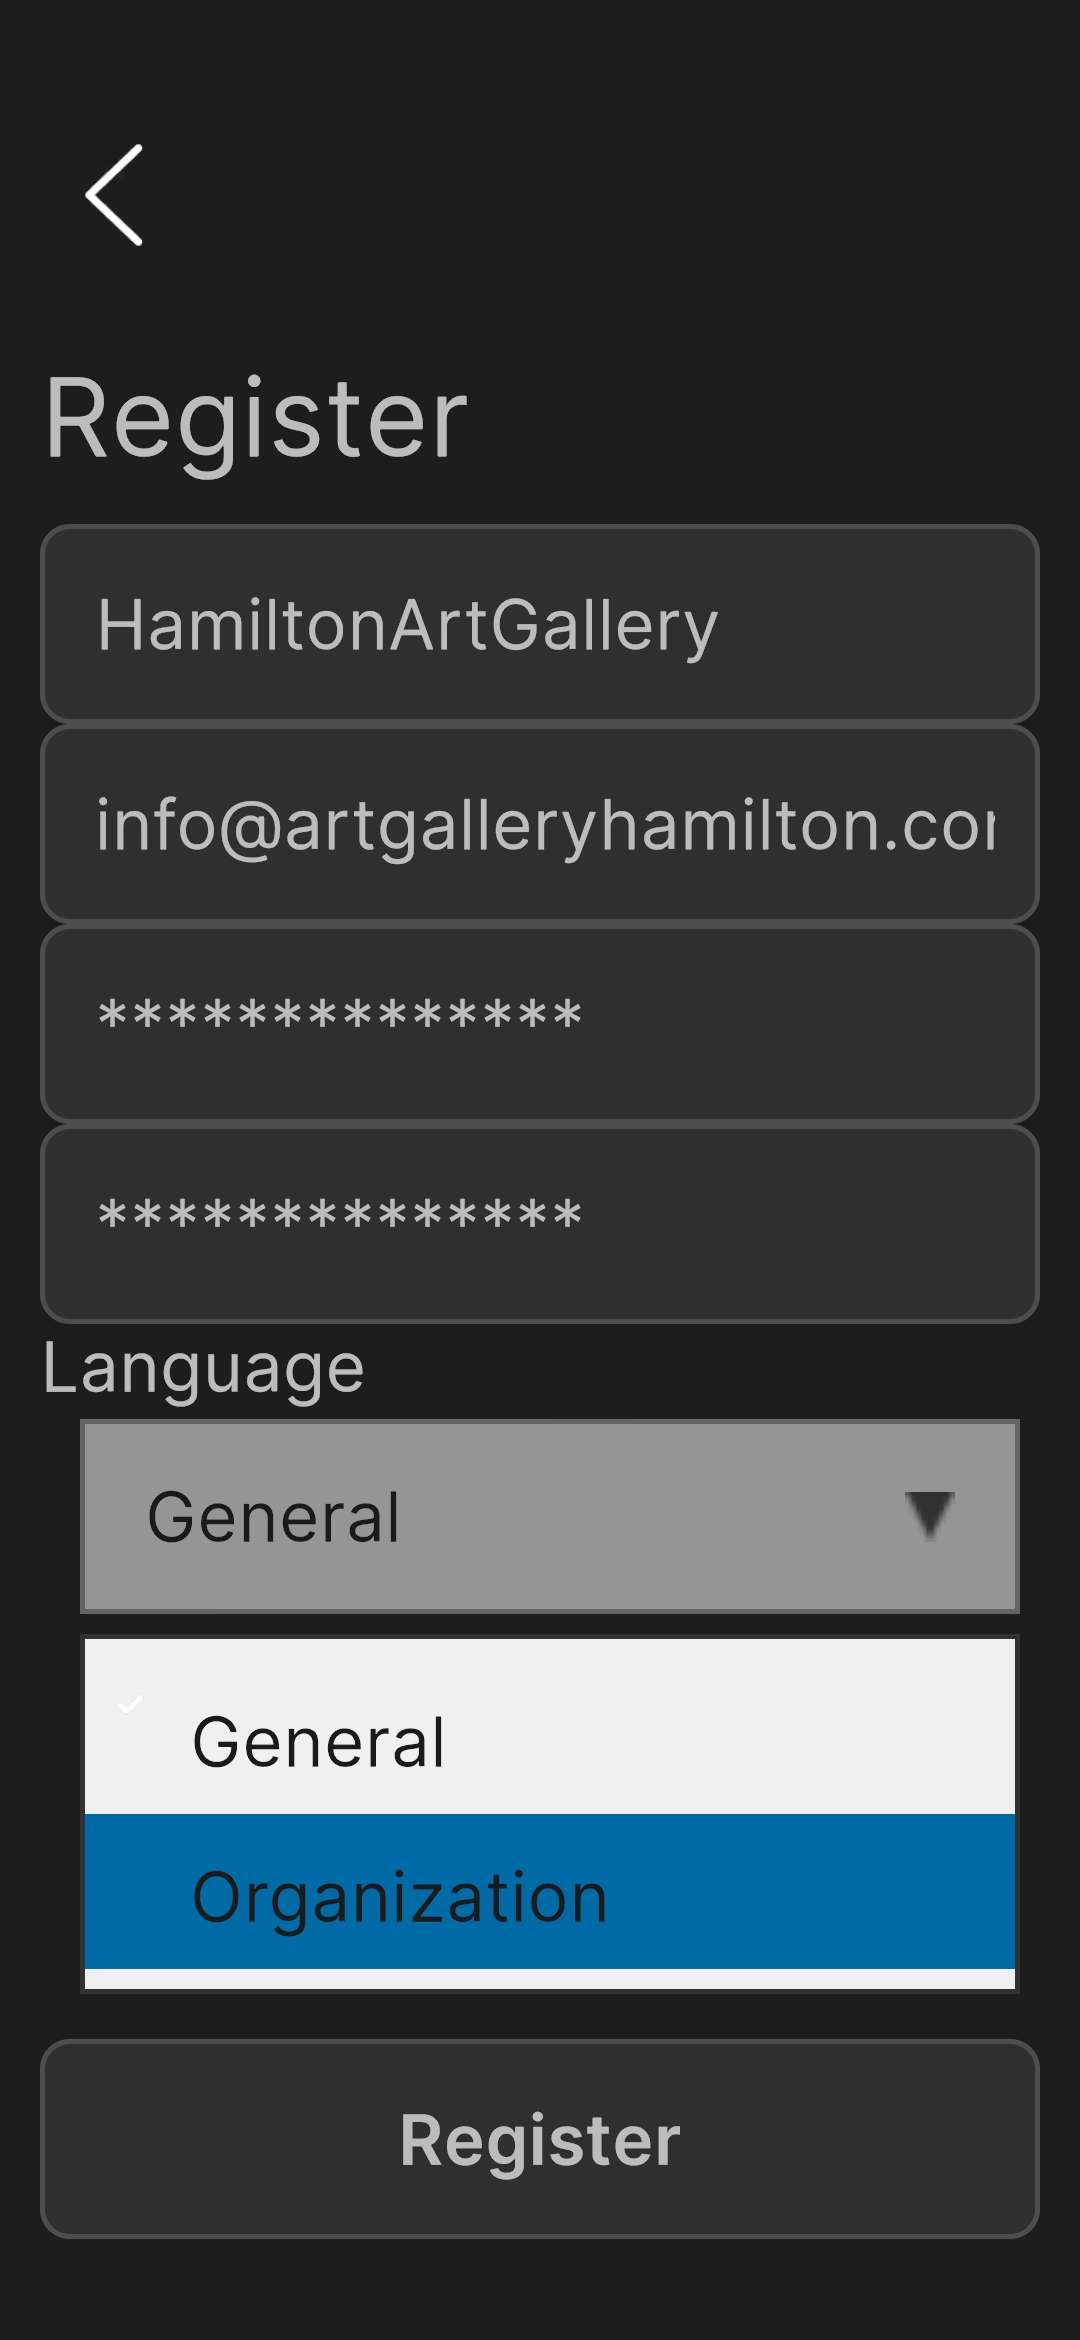
\includegraphics[width=\textwidth]{register3.png}
    \end{subfigure}
    \caption{Filling Required Fields}
    \label{fig:setup2}
\end{figure}

\newpage
\begin{figure}[ht!]
    \centering
    \begin{subfigure}[b]{0.48\textwidth}
        \centering
        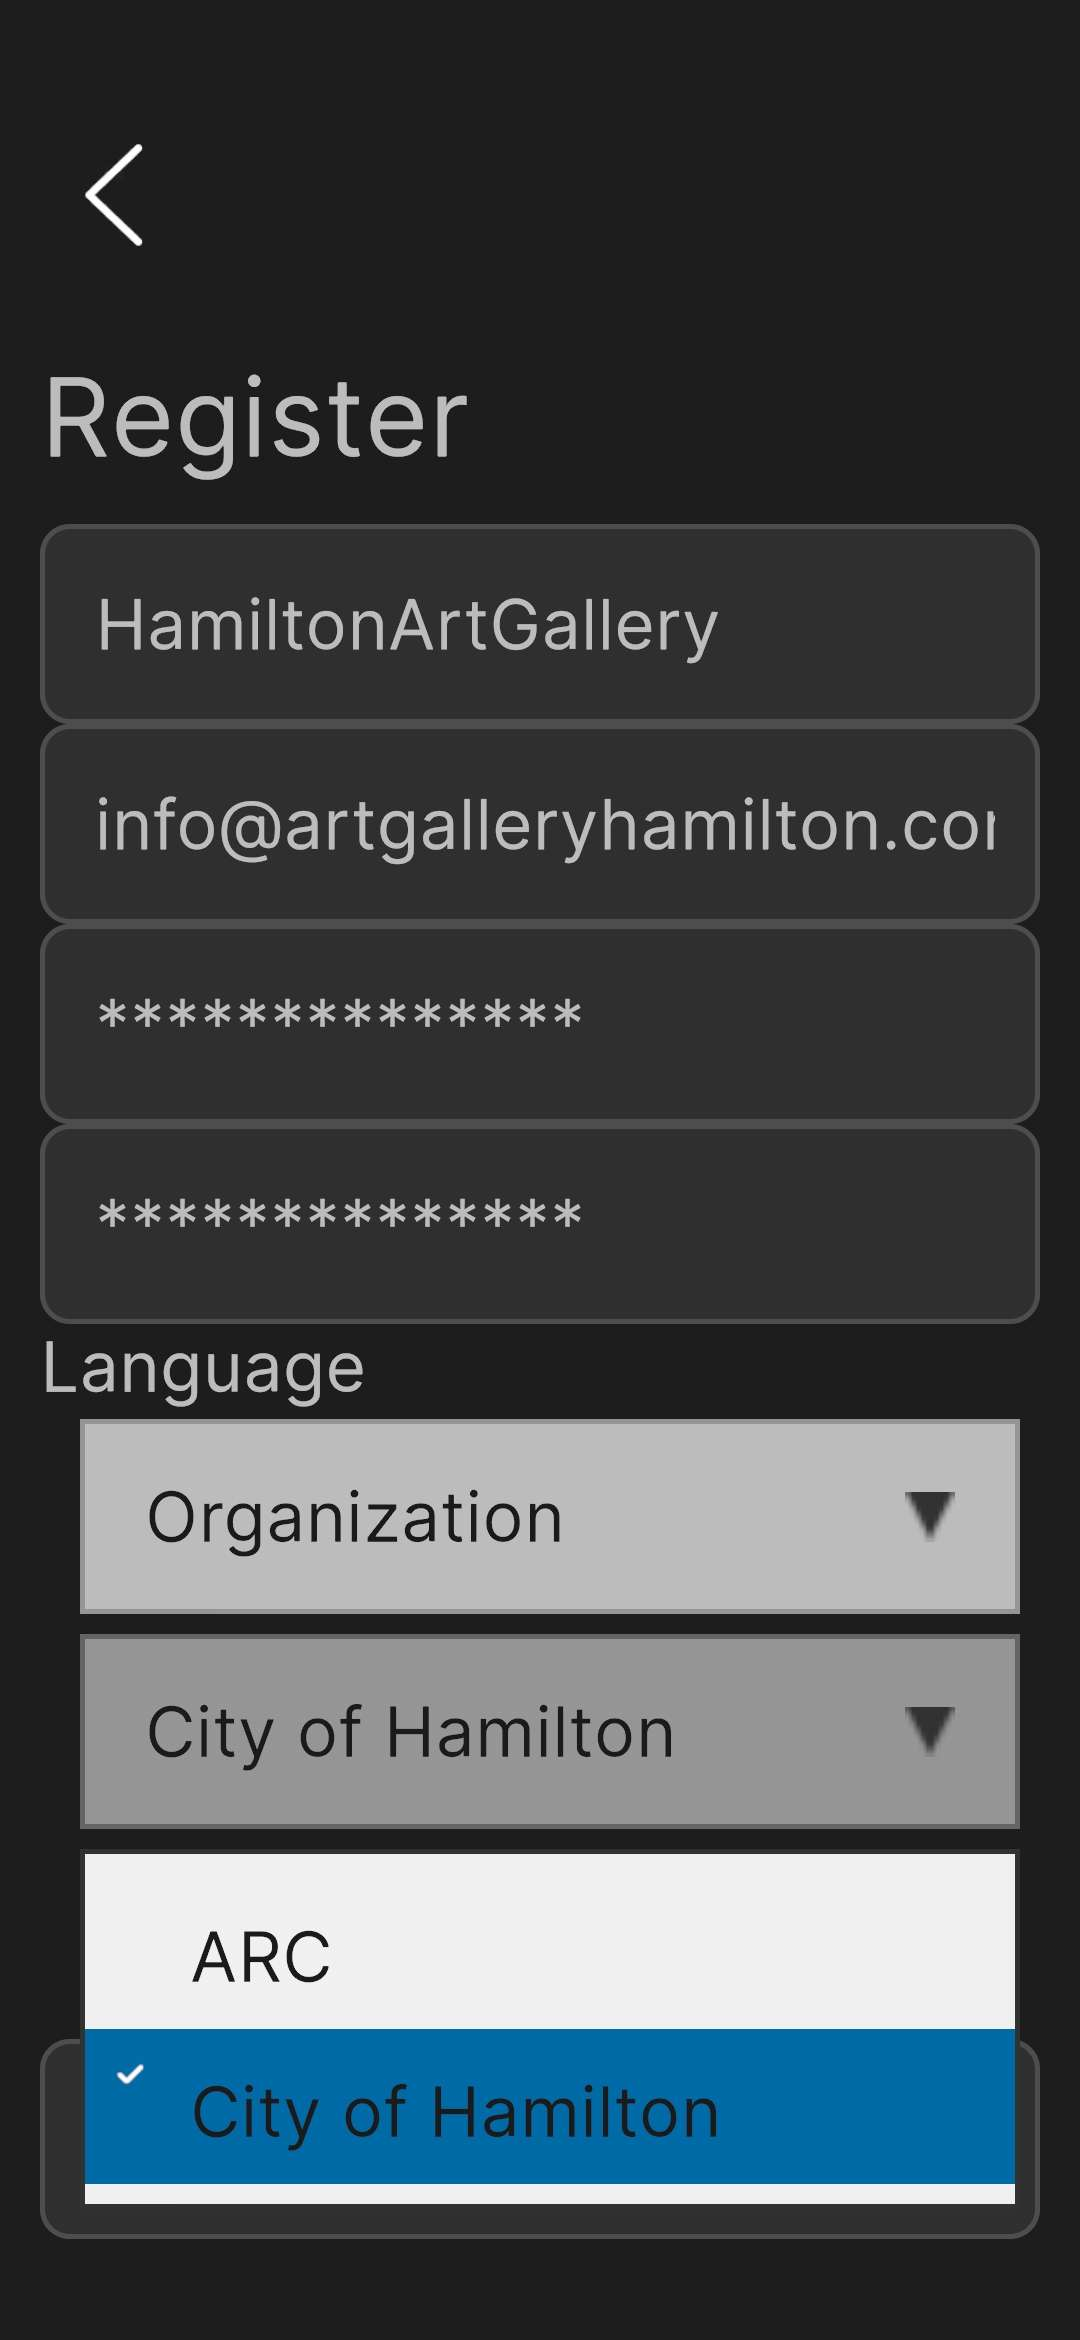
\includegraphics[width=\textwidth]{register4.png}
    \end{subfigure}
    \hfill
    \begin{subfigure}[b]{0.48\textwidth}
        \centering
        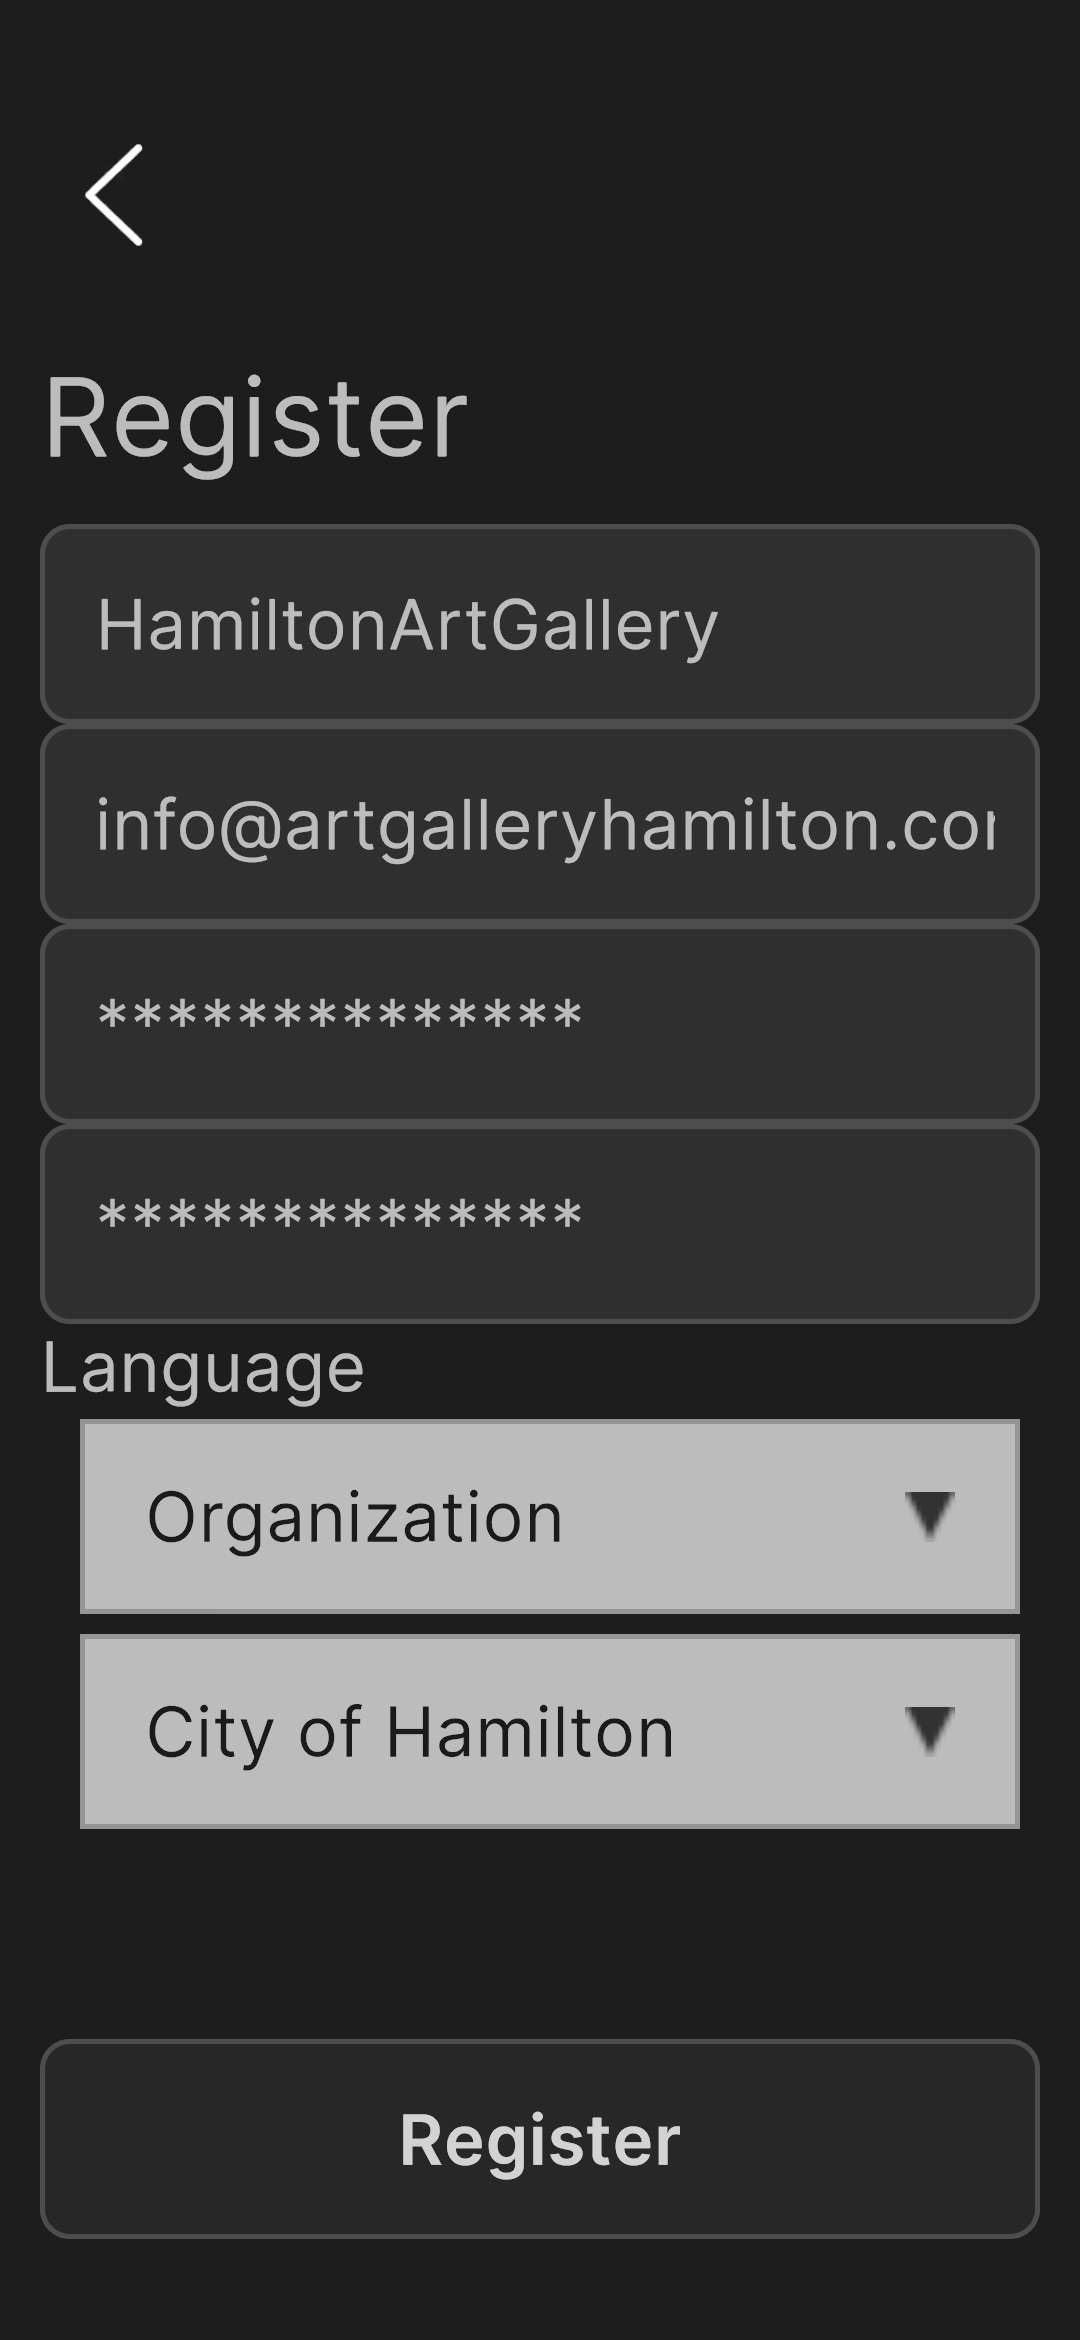
\includegraphics[width=\textwidth]{register5.png}
    \end{subfigure}
    \caption{Selecting User Type and Completing Registration}
    \label{fig:setup3}
\end{figure}

%-----------------------------

\clearpage
\section{Overview of the User Interface}
\subsection{\texttt{Tour List} Screen Layout}
The \texttt{Tour List} screen is the main interface for users to view and select available tours. Users can access the \hyperref[fig:maps]{Maps} screen from here as well.

\begin{figure}[ht!]
    \setlength{\fboxrule}{0.1mm}
    \centering
    \fbox{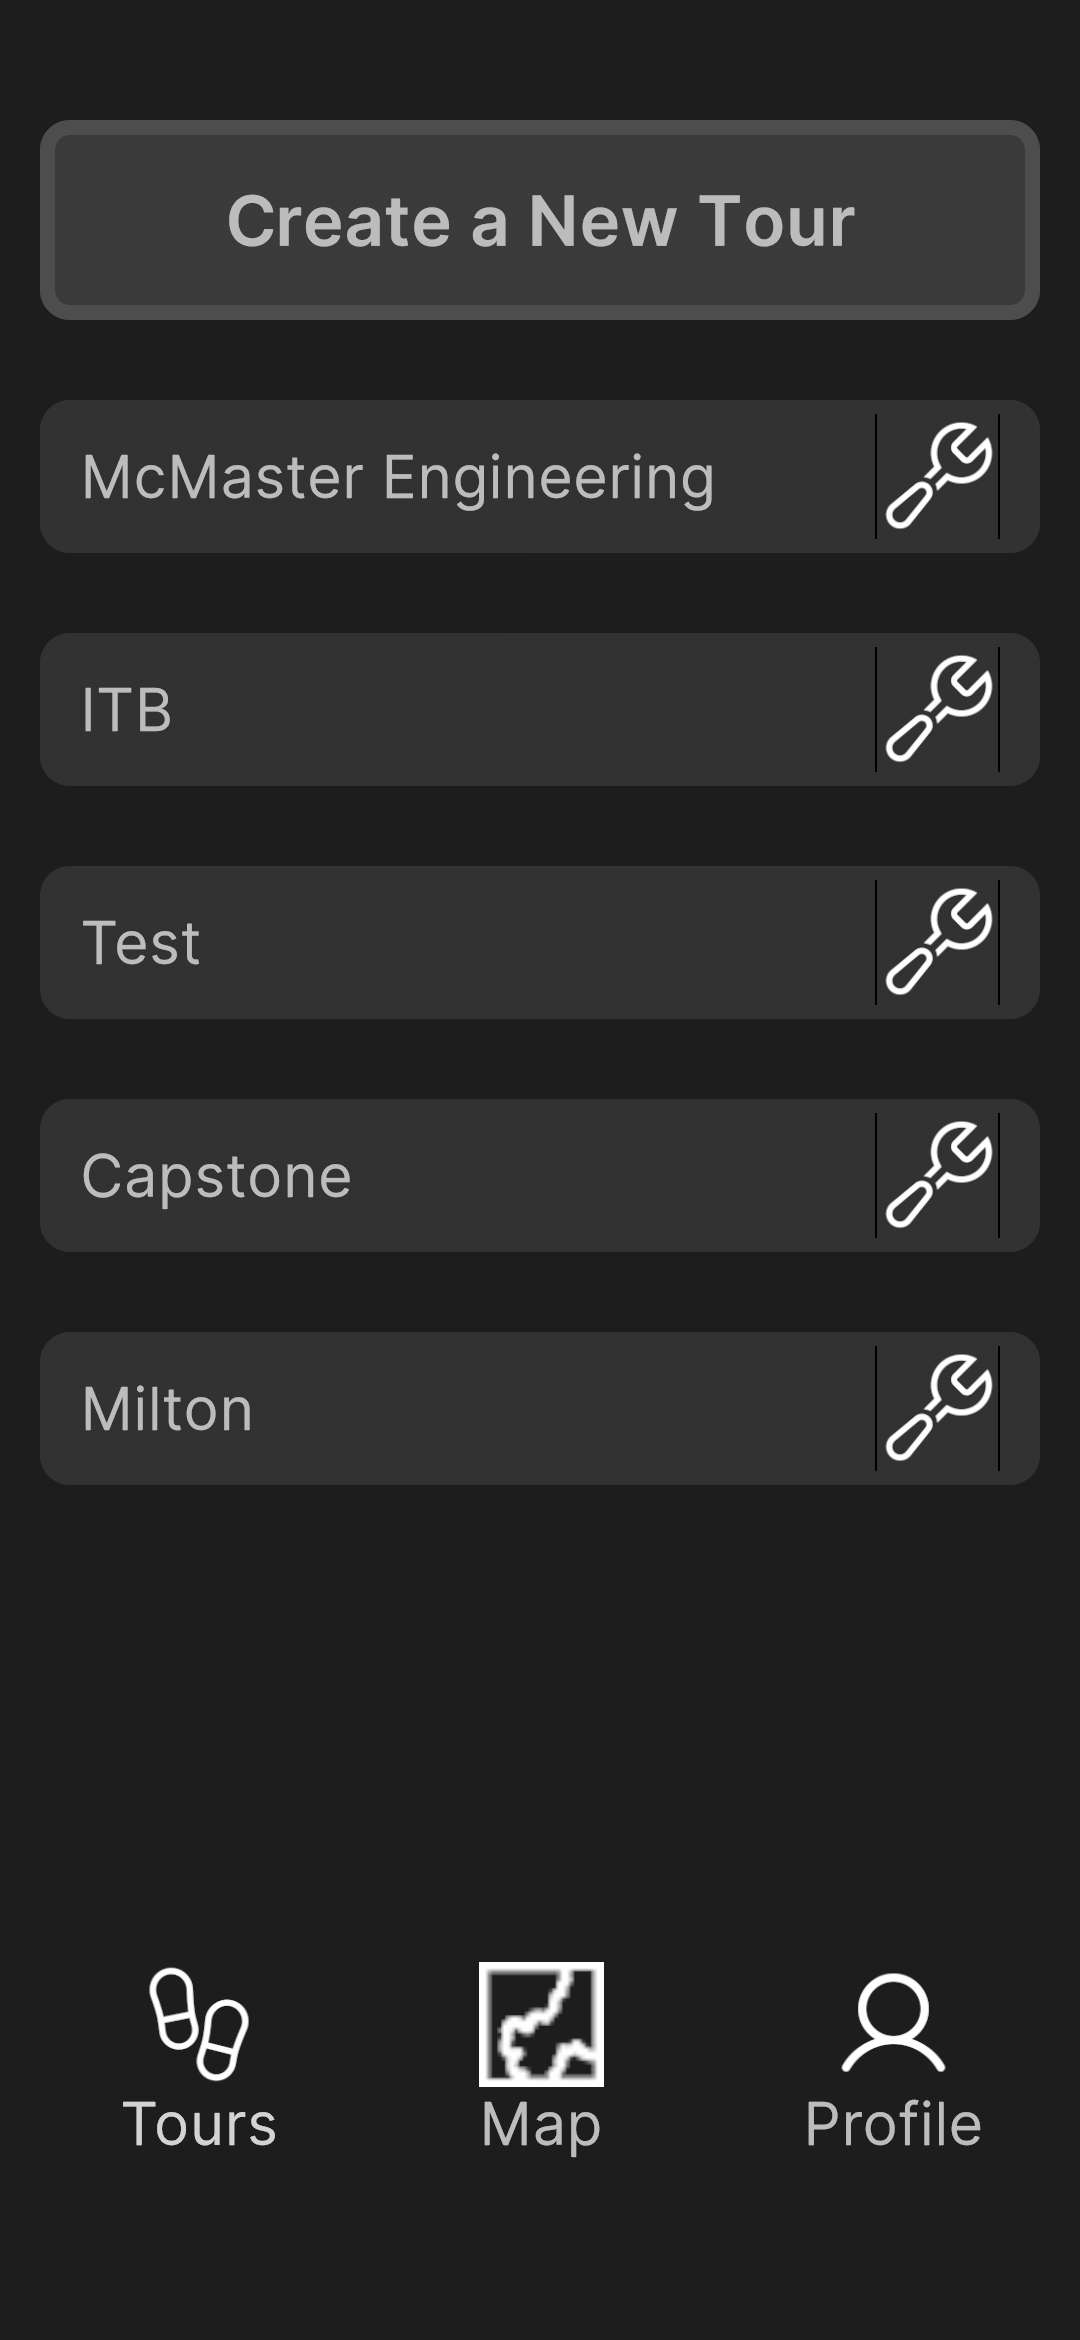
\includegraphics[width=0.5\textwidth]{tour_screen.png}}
    \caption{Tour List Screen of \progname{}}
    \label{fig:tours}
\end{figure}

\newpage
\subsection{\texttt{Map} Screen Layout}
The \texttt{Map} screen provides an interactive map view of the user's current location and nearby tours. It includes features such as zooming, panning, and selecting markers to view tour details. The user can also recenter the map to their current location via the bottom left button.

\begin{figure}[ht!]
    \setlength{\fboxrule}{0.1mm}
    \centering
    \fbox{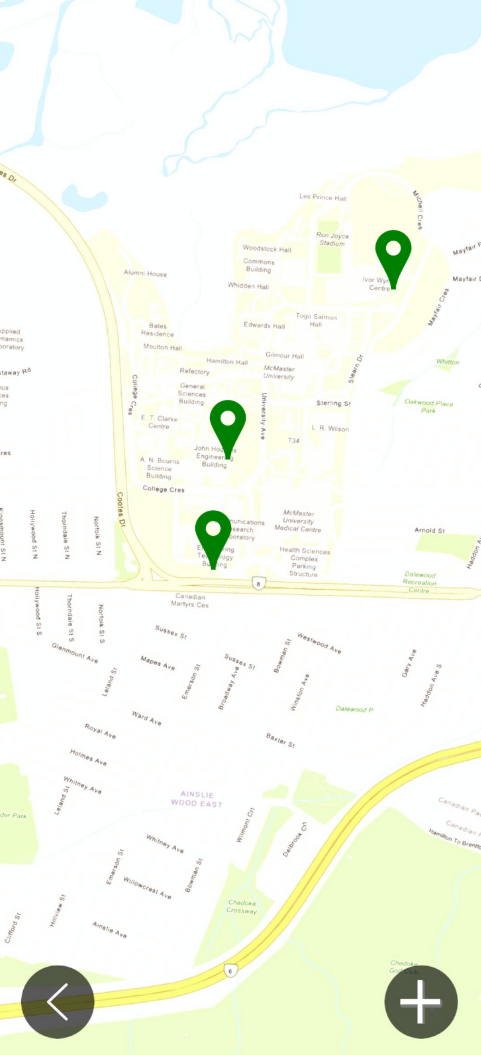
\includegraphics[width=0.5\textwidth]{map_screen.png}}
    \caption{Map Screen of \progname{}}
    \label{fig:maps}
\end{figure}

\subsection{Login Screen Layout}
The \texttt{Login} screen is where users enter their credentials to access the app. It includes fields for email and password, as well as options for account creation.

\begin{figure}[ht!]
    \setlength{\fboxrule}{0.1mm}
    \centering
    \fbox{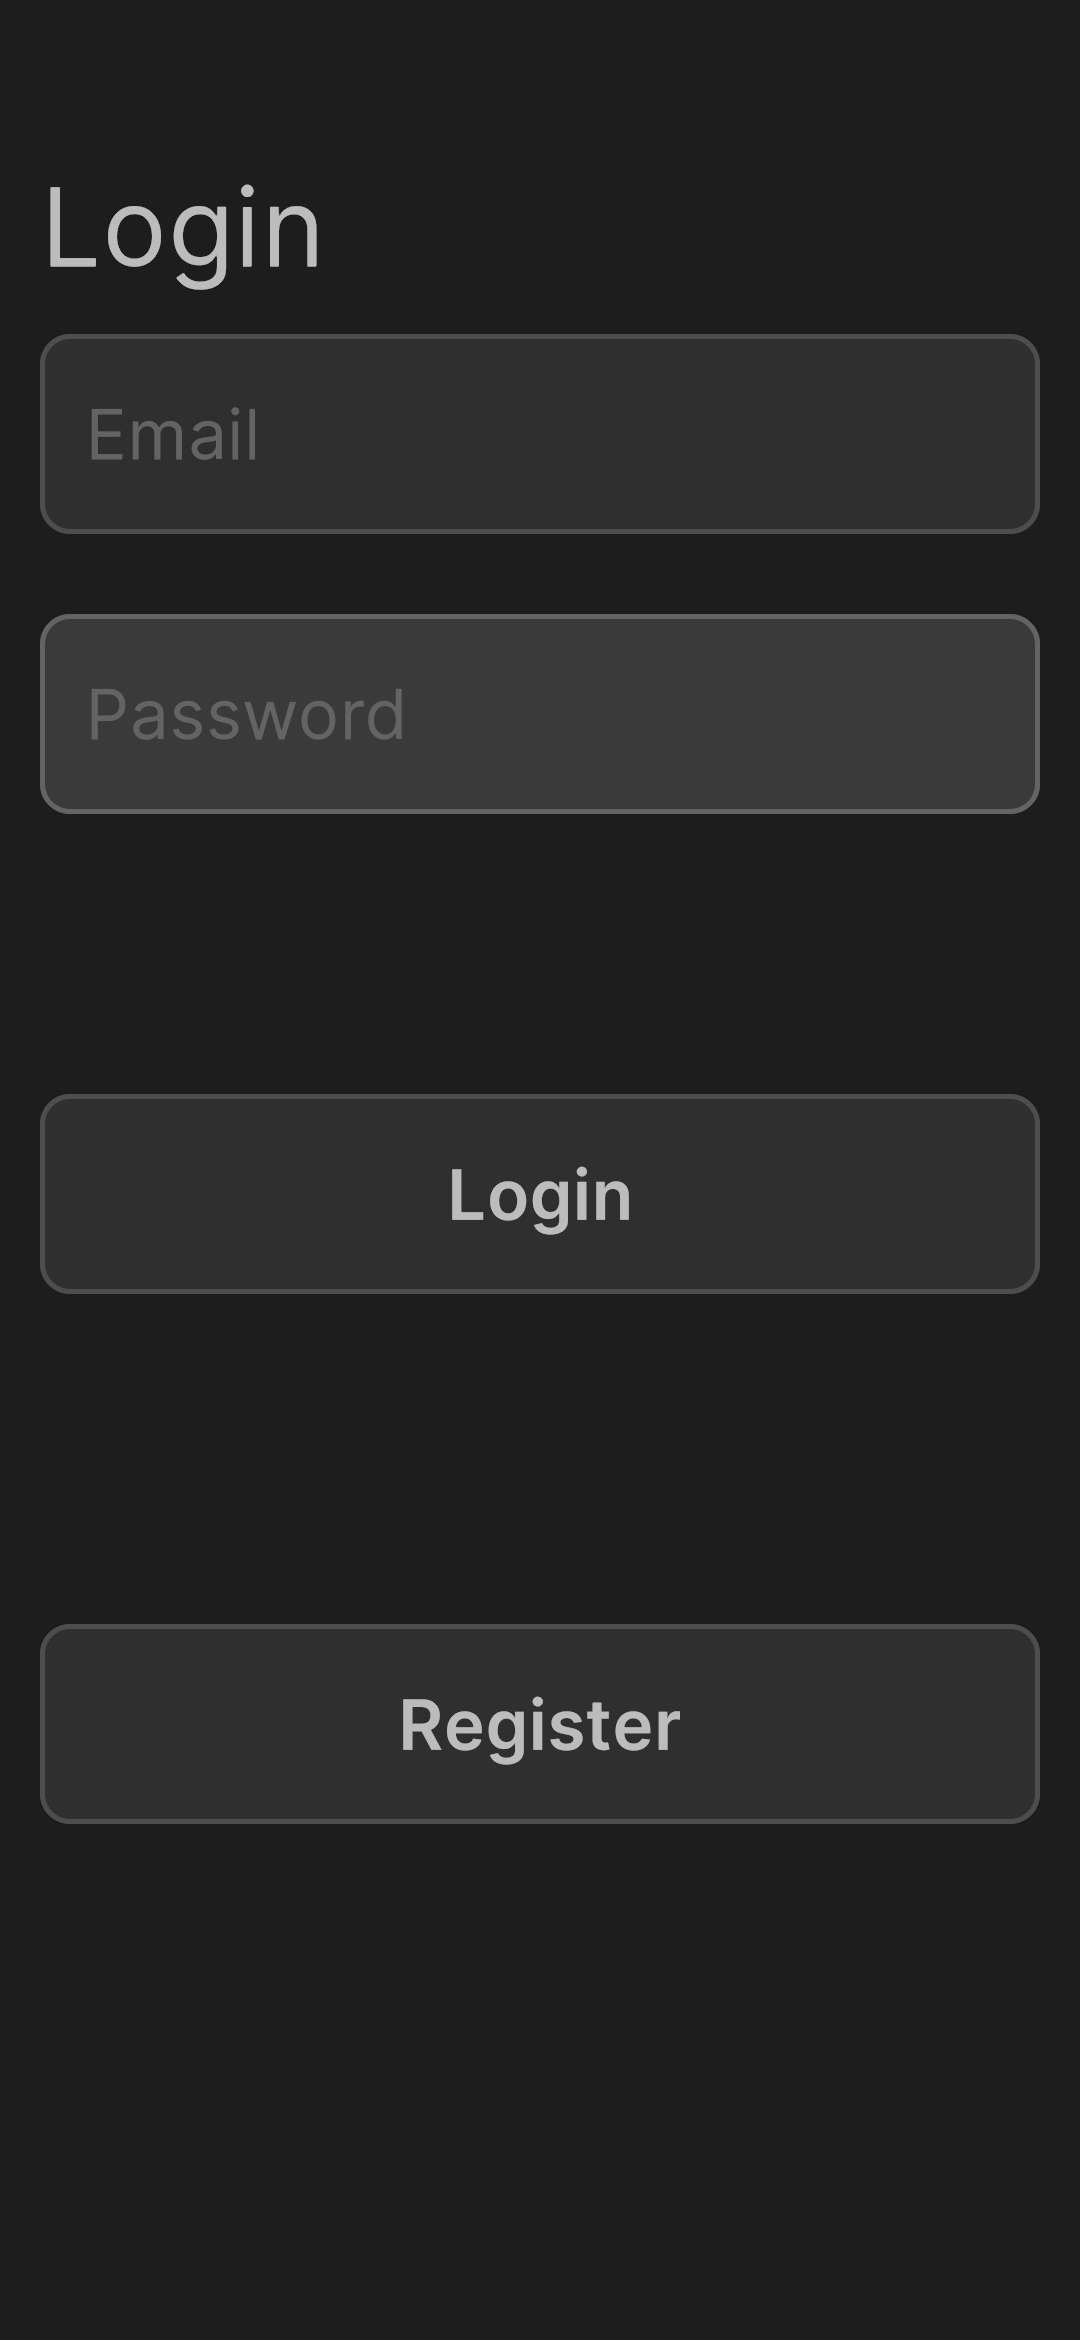
\includegraphics[width=0.5\textwidth]{login1.png}}
    \caption{Login Screen of \progname{}}
    \label{fig:login1}
\end{figure}

\subsection{Navigation}
Users can navigate through the app using the bottom navigation bar, which includes icons for \texttt{Tours}, \texttt{Map}, and \texttt{Profile}. Tapping on each icon will take the user to the corresponding screen.

\begin{figure}[ht!]
    \centering
    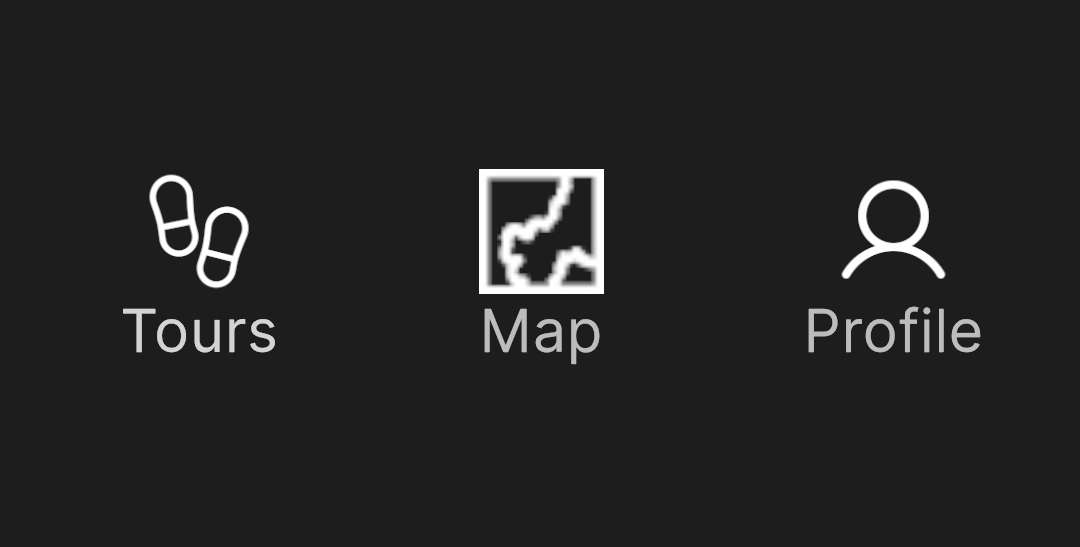
\includegraphics[width=0.5\textwidth]{nav_bar.png}
    \caption{Bottom Navigation Bar of \progname{}}
    \label{fig:nav_bar}
\end{figure}

%-----------------------------
\section{Features and Functionalities}
The following subsections detail the key features and functionalities of \textbf{\progname{}}. Each section includes an overview, purpose and step-by-step instructions. The goal is to provide clear and concise guidance for users to effectively utilize the app's capabilities.

\subsection{Viewing a Tour}
\textbf{Overview:} This feature enables General users to experience AR tours created by Organizational users. It offers an interactive preview of tour details along with both AR and map-based navigation.

\textbf{Key Features:}
\begin{itemize}[leftmargin=*]
    \item \textbf{Tour Preview:} Displays the tour's name and description and if applicable, additional content like historical information.
    \item \textbf{Viewing AR objects:} Users can view AR objects in the real world by pointing their device's camera at the designated area.
    \item \textbf{Navigation Assistance:} Provides on-screen directions, showing the intended route and nearby AR objects.
\end{itemize}

\textbf{How to Use:}
\begin{enumerate}[leftmargin=*]
    \item Open the \emph{Tours} section from the main menu.
    \item Select a tour from the list to view its details.
    \item Tap \emph{Start} to start the tour.
    \item Use the AR view for an immersive experience.
    \item Follow the guided steps until the tour is completed, then exit to return to the tour list.
\end{enumerate}

\begin{figure}[ht!]
    \centering
    \begin{subfigure}[b]{0.48\textwidth}
        \centering
        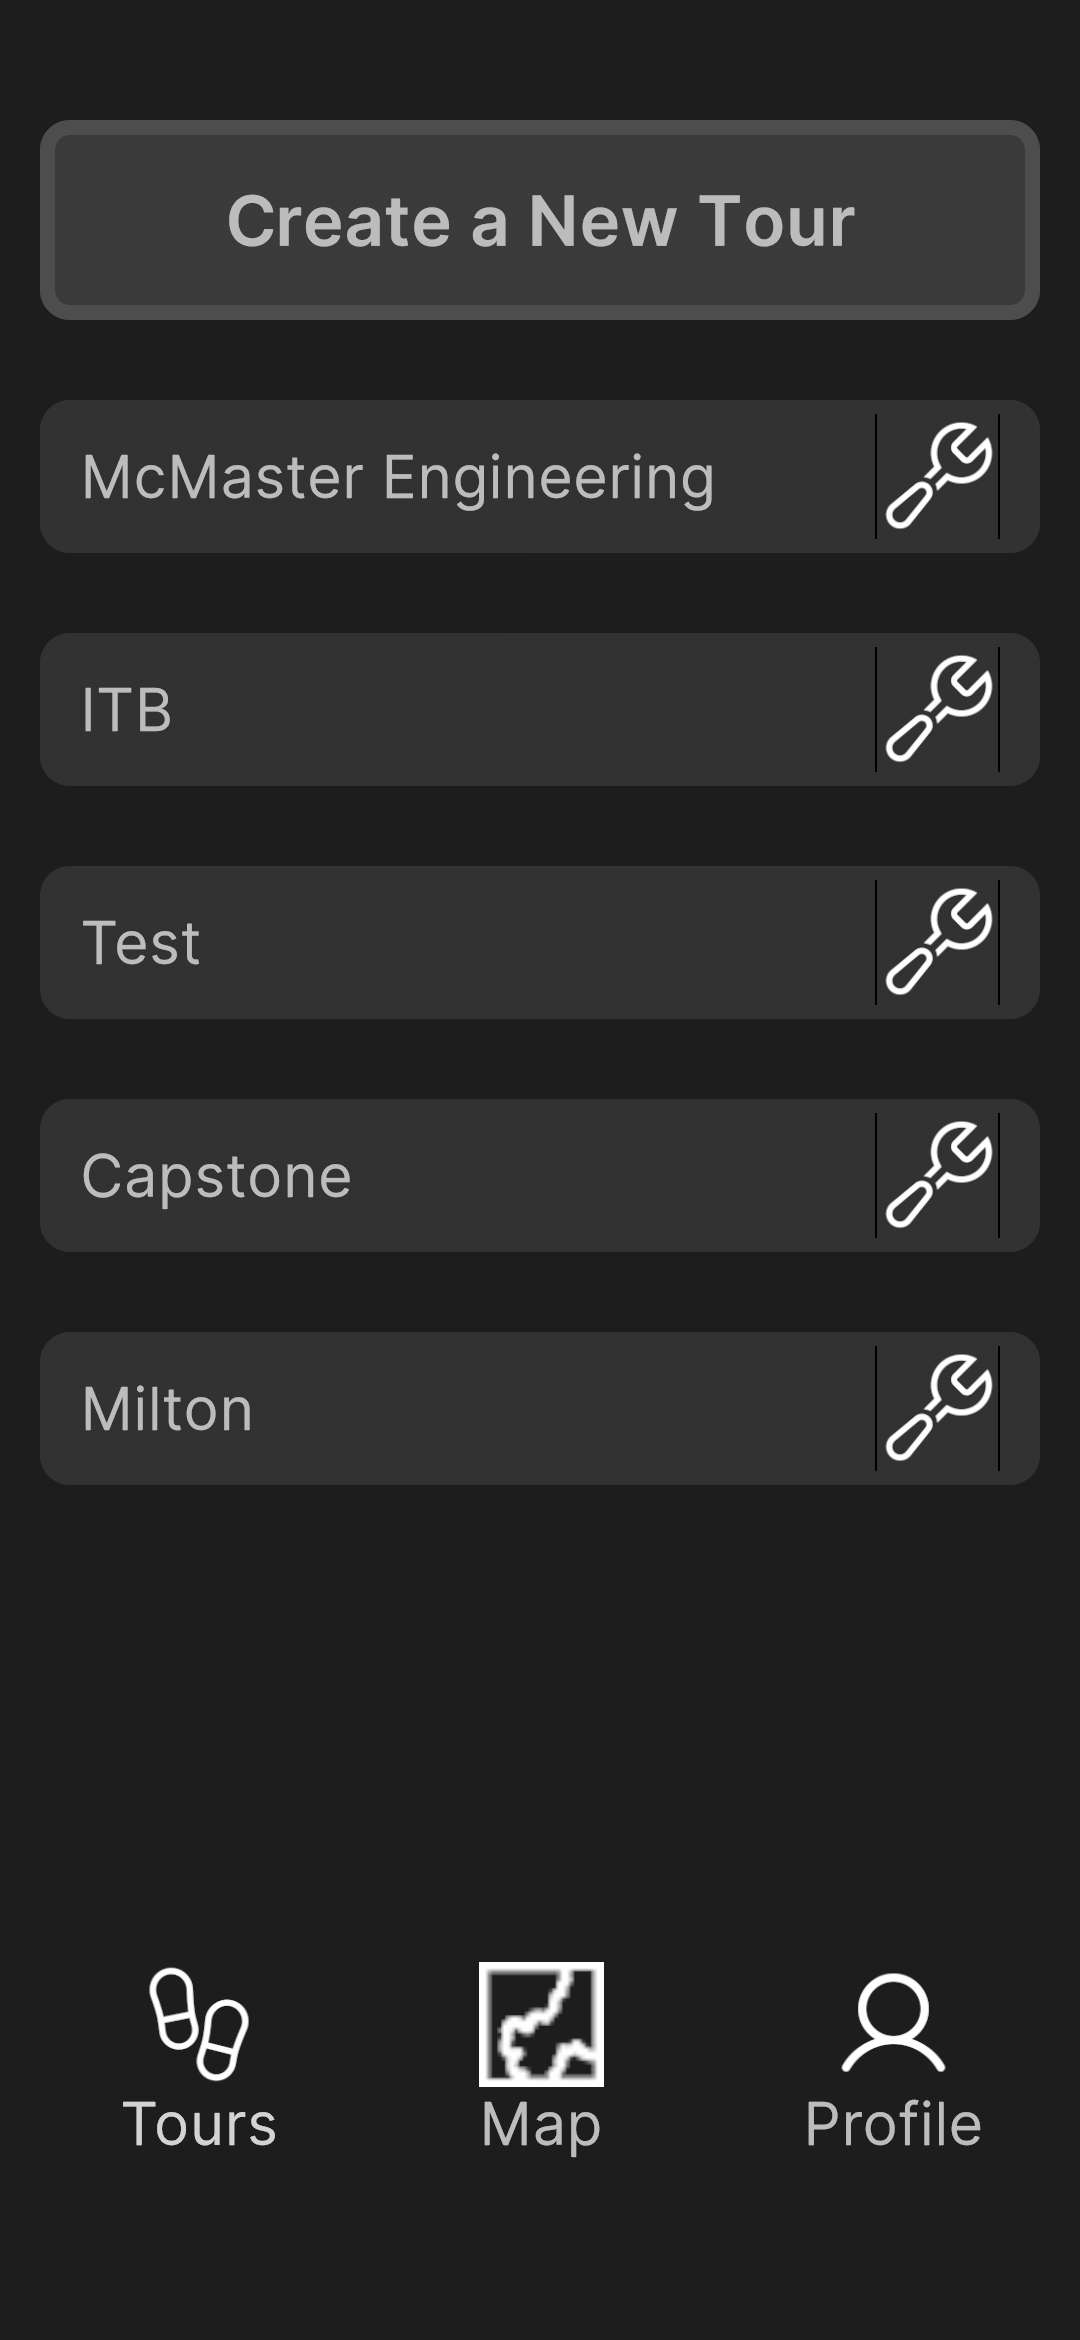
\includegraphics[width=\textwidth]{tour_screen.png}
    \end{subfigure}
    \hfill
    \begin{subfigure}[b]{0.48\textwidth}
        \centering
        
\includegraphics[width=\textwidth]{start_tour.png}
    \end{subfigure}
    \caption{Starting a Tour}
    \label{fig:tourview1}
\end{figure}

\newpage
\subsection{Creating a Tour}
\textbf{Overview:} Available only to Organizational users, this feature allows the creation, editing, and management of AR tours. Tours can initially be saved as drafts and later published for General users.

\textbf{Key Features:}
\begin{itemize}[leftmargin=*]
    \item \textbf{Tour Details Form:} Input essential details such as the tour name and description.
    \item \textbf{Route Configuration:} Define the tour area on an interactive map; set the route, intended direction, and estimated time of completion.
    \item \textbf{Inventory Setup:} Upload or generate AR objects to be placed along the tour route.
    \item \textbf{Publish Options:} Choose to save the tour to make it visible to General users.
\end{itemize}

\textbf{How to Use:}
\begin{enumerate}[leftmargin=*]
    \item Navigate to the \emph{Tour List} main interface.
    \item Select \emph{Create a New Tour} and fill in the tour details form.
    \item Set up the inventory by uploading or generating AR objects along the route.
    \item \hyperref[fig:obj_place]{Place} the AR objects in the desired locations around the route.
    \item Review the complete tour and choose to save it.
    \item Optionally, the Organizational user can \hyperref[fig:edit_tour]{edit} an existing tour by clicking on the Edit icon next to the tour name in the \emph{Tour List} screen.
\end{enumerate}

\begin{figure}[ht!]
    \centering
    \begin{subfigure}[b]{0.48\textwidth}
        \centering
        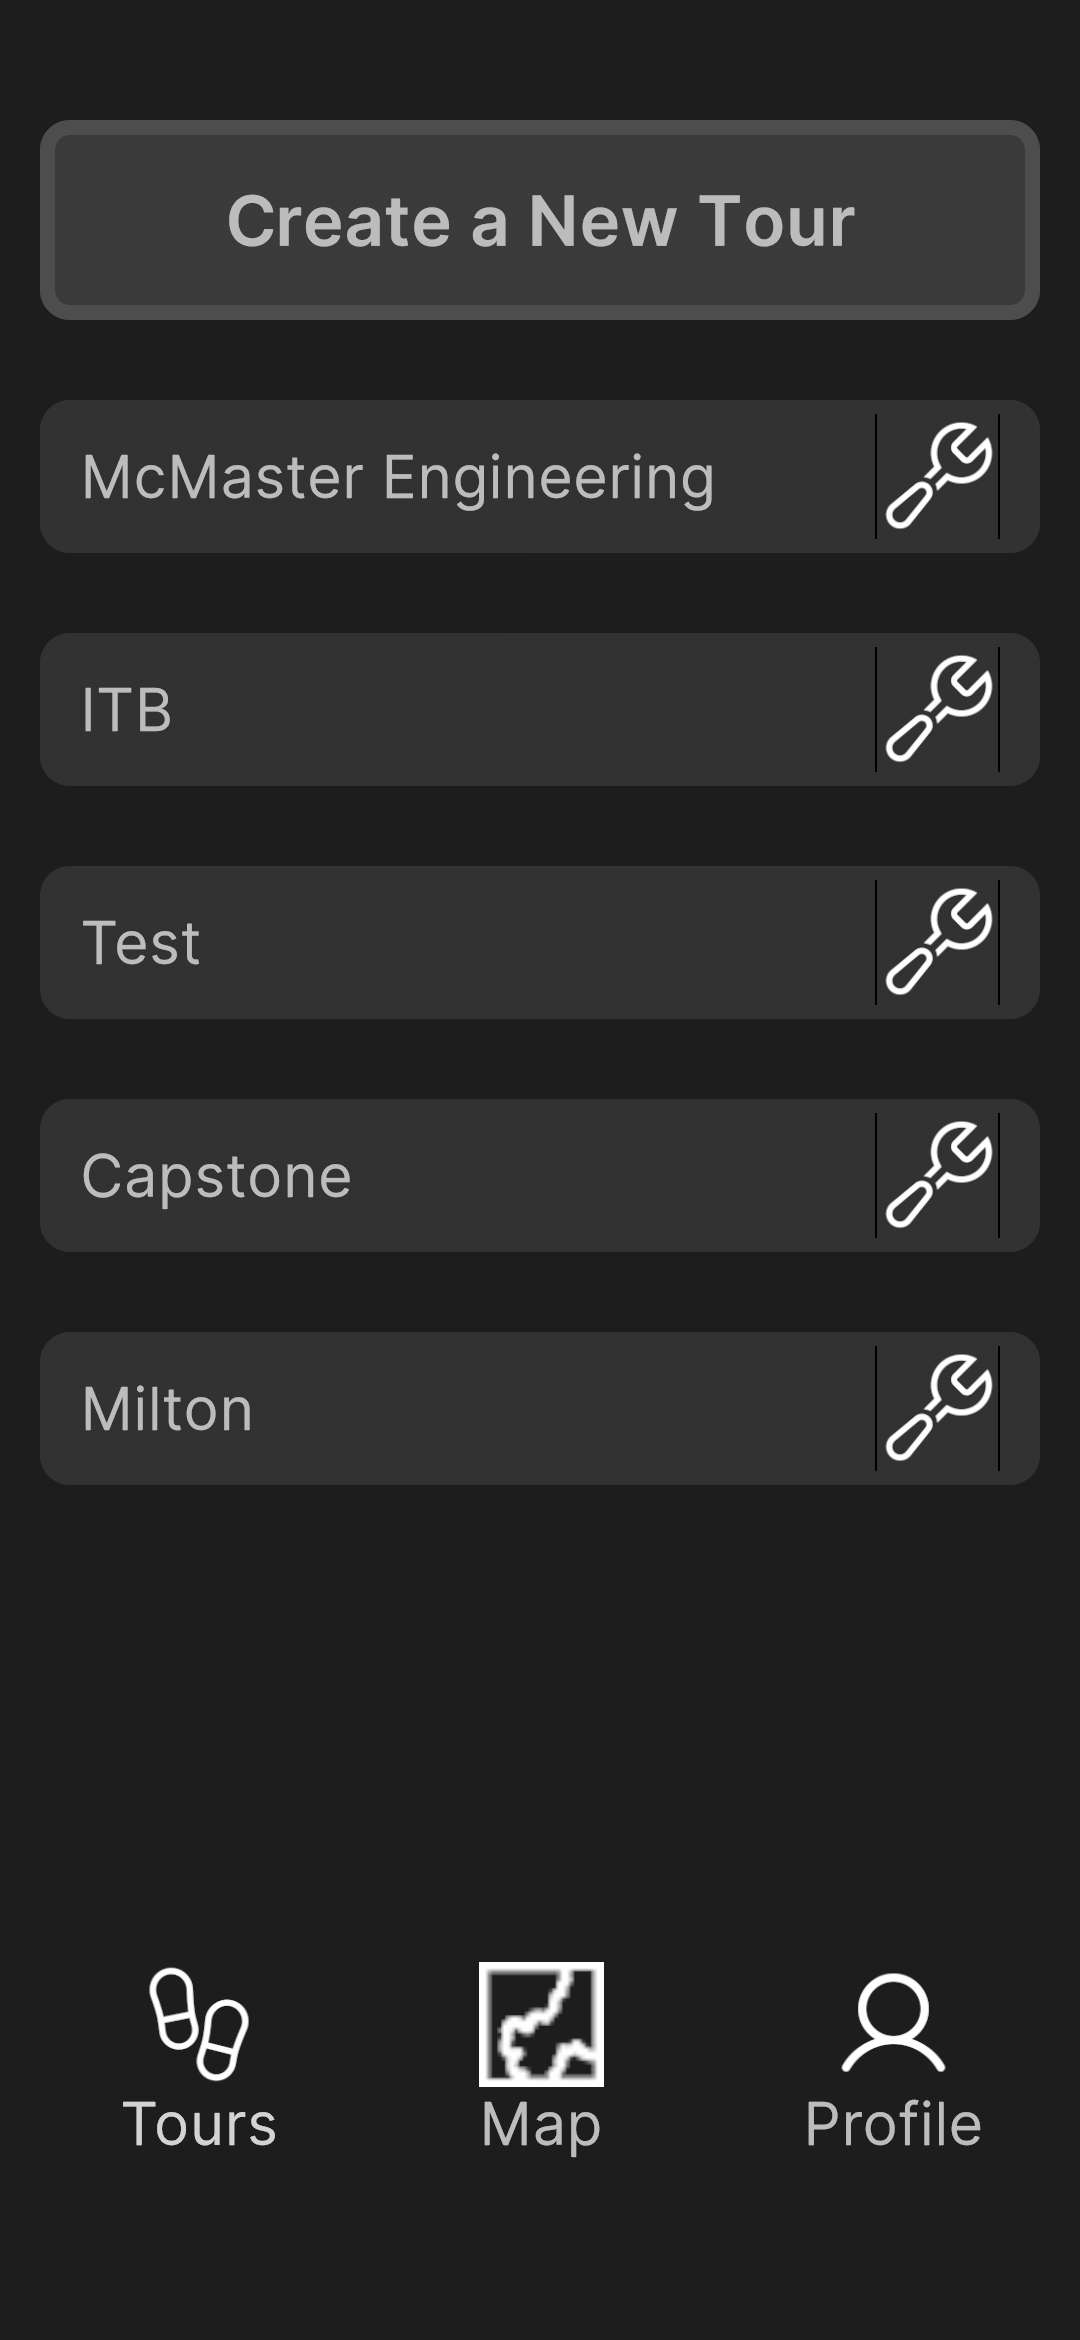
\includegraphics[width=\textwidth]{tour_screen.png}
    \end{subfigure}
    \hfill
    \begin{subfigure}[b]{0.48\textwidth}
        \centering
        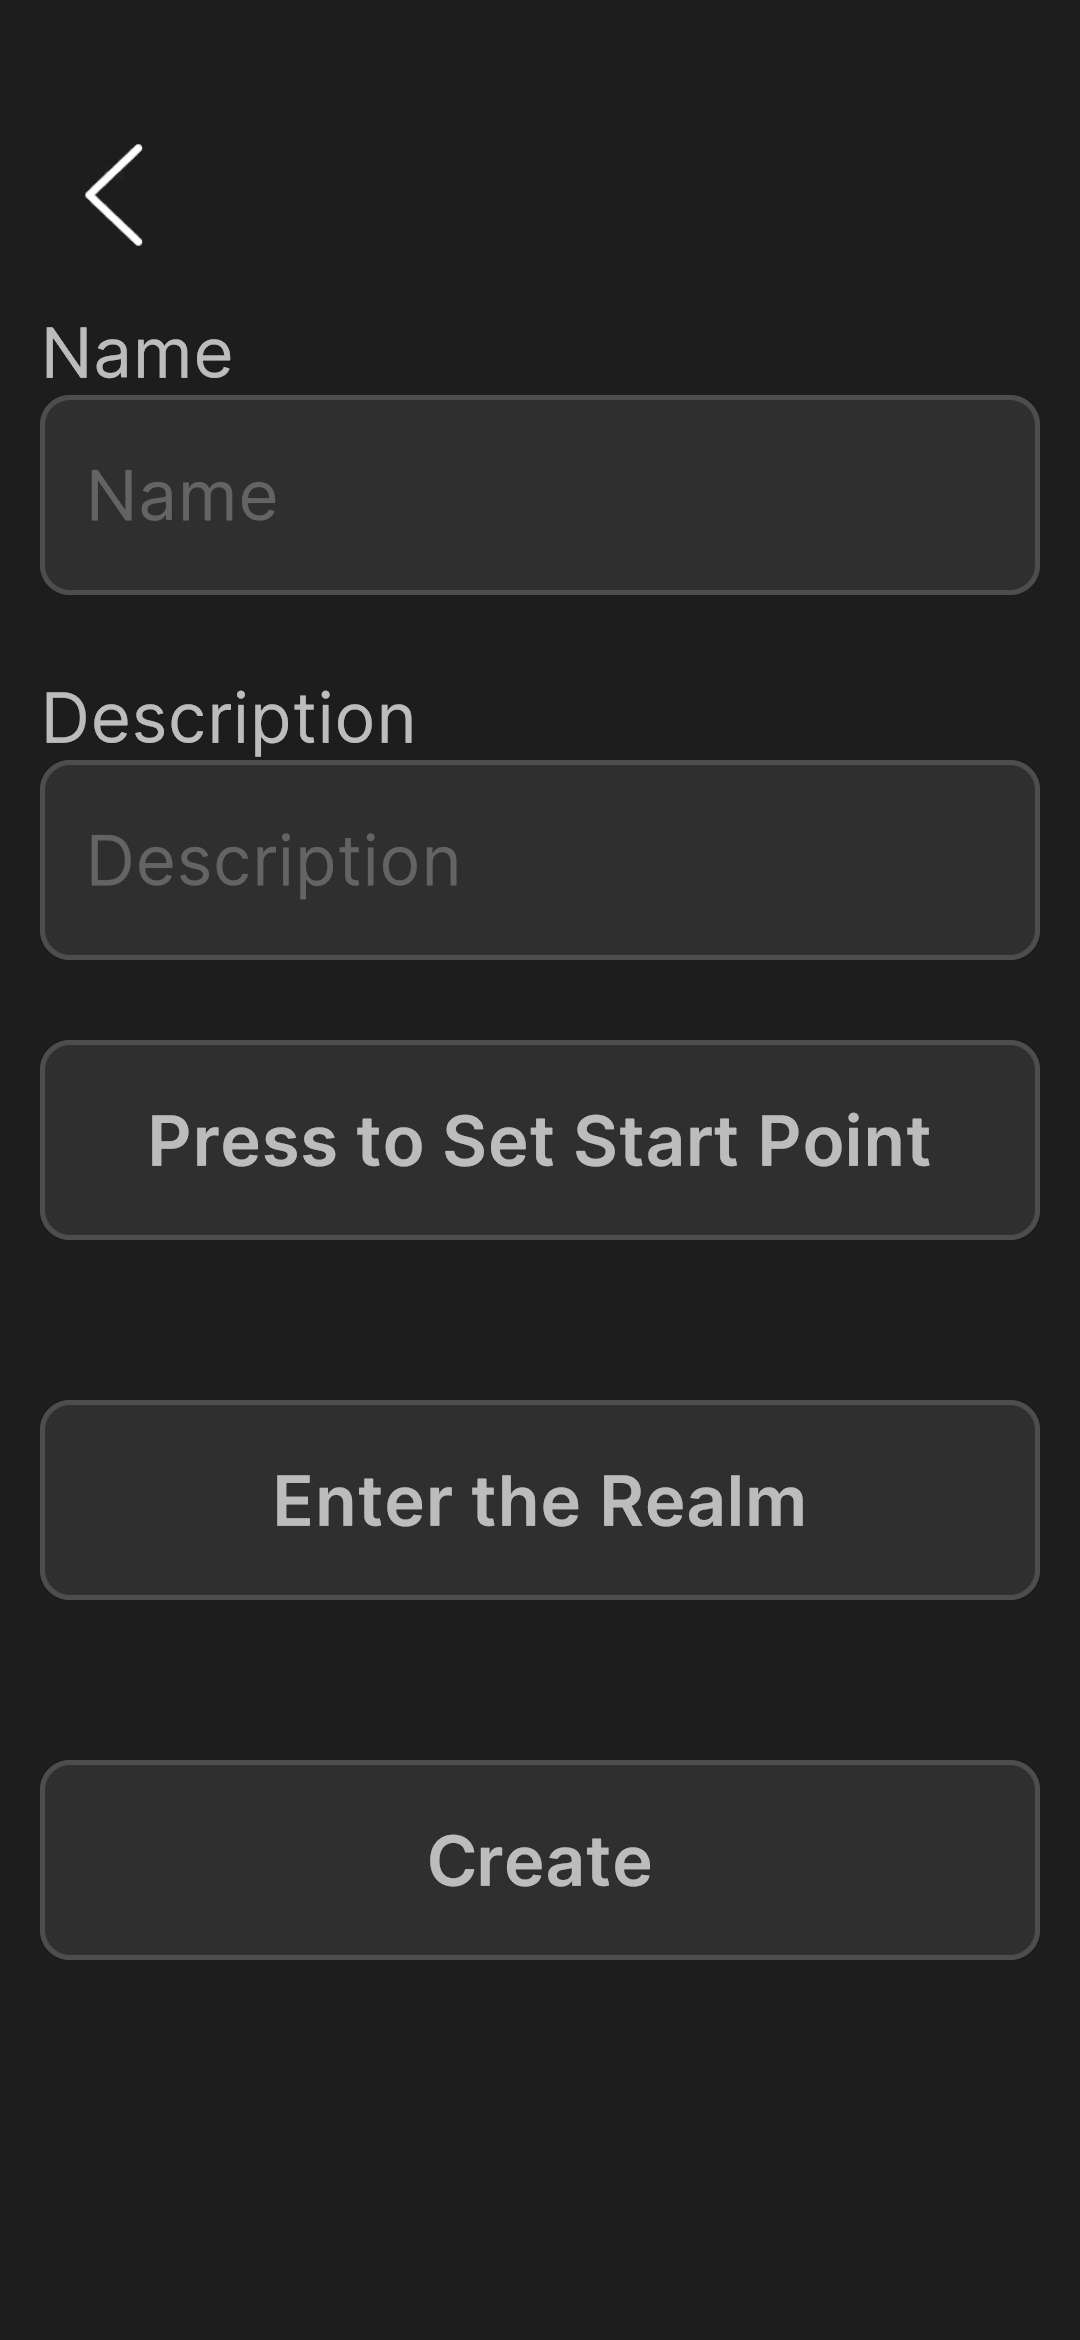
\includegraphics[width=\textwidth]{create_tour.png}
    \end{subfigure}
    \caption{Creating a Tour as an Organizational User}
    \label{fig:createtour}
\end{figure}

\newpage
\begin{figure}[ht!]
    \centering
    \begin{subfigure}[b]{0.48\textwidth}
        \centering
        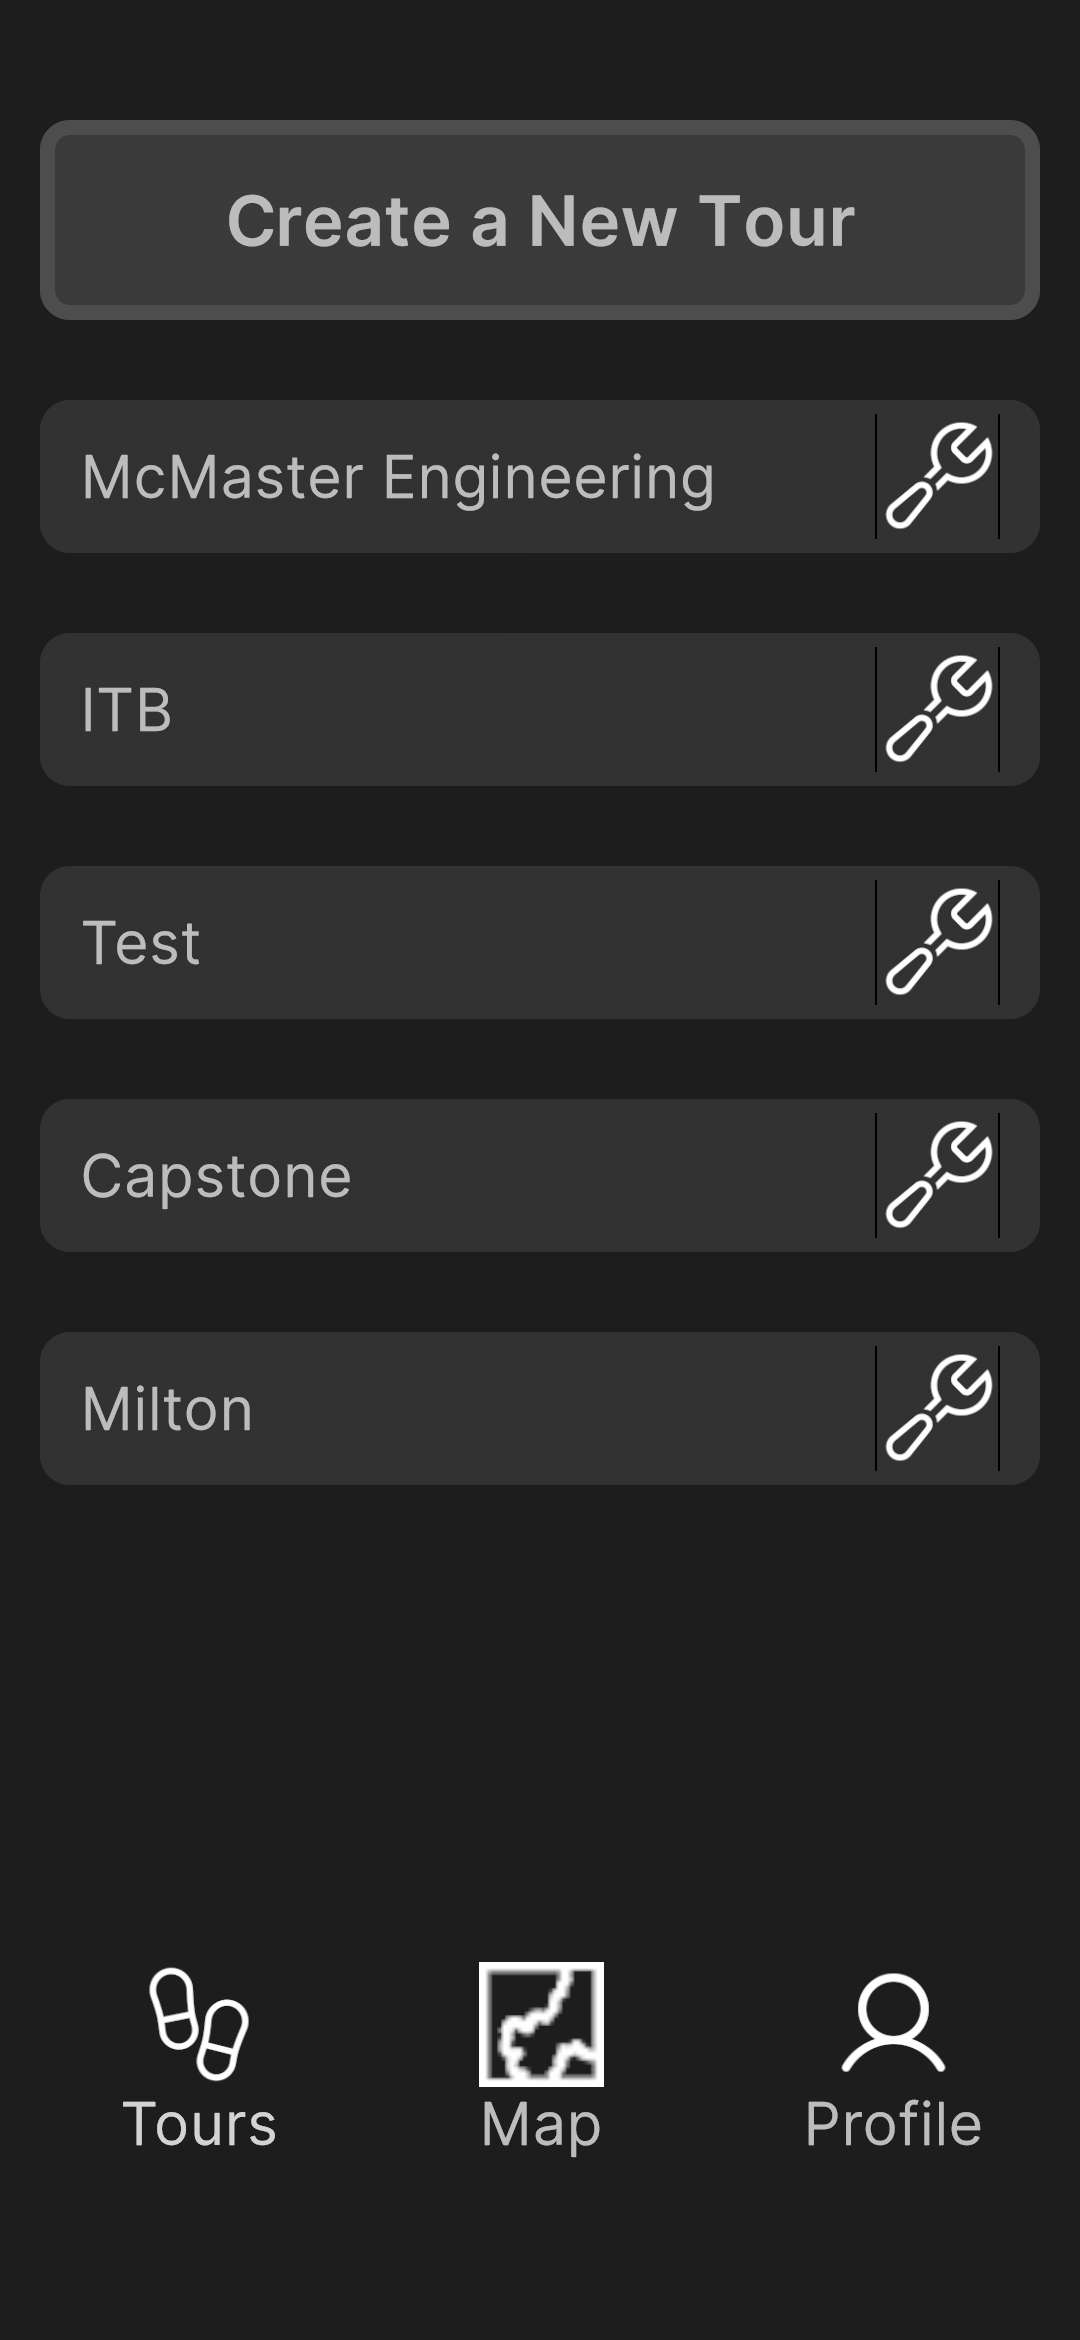
\includegraphics[width=\textwidth]{tour_screen.png}
    \end{subfigure}
    \hfill
    \begin{subfigure}[b]{0.48\textwidth}
        \centering
        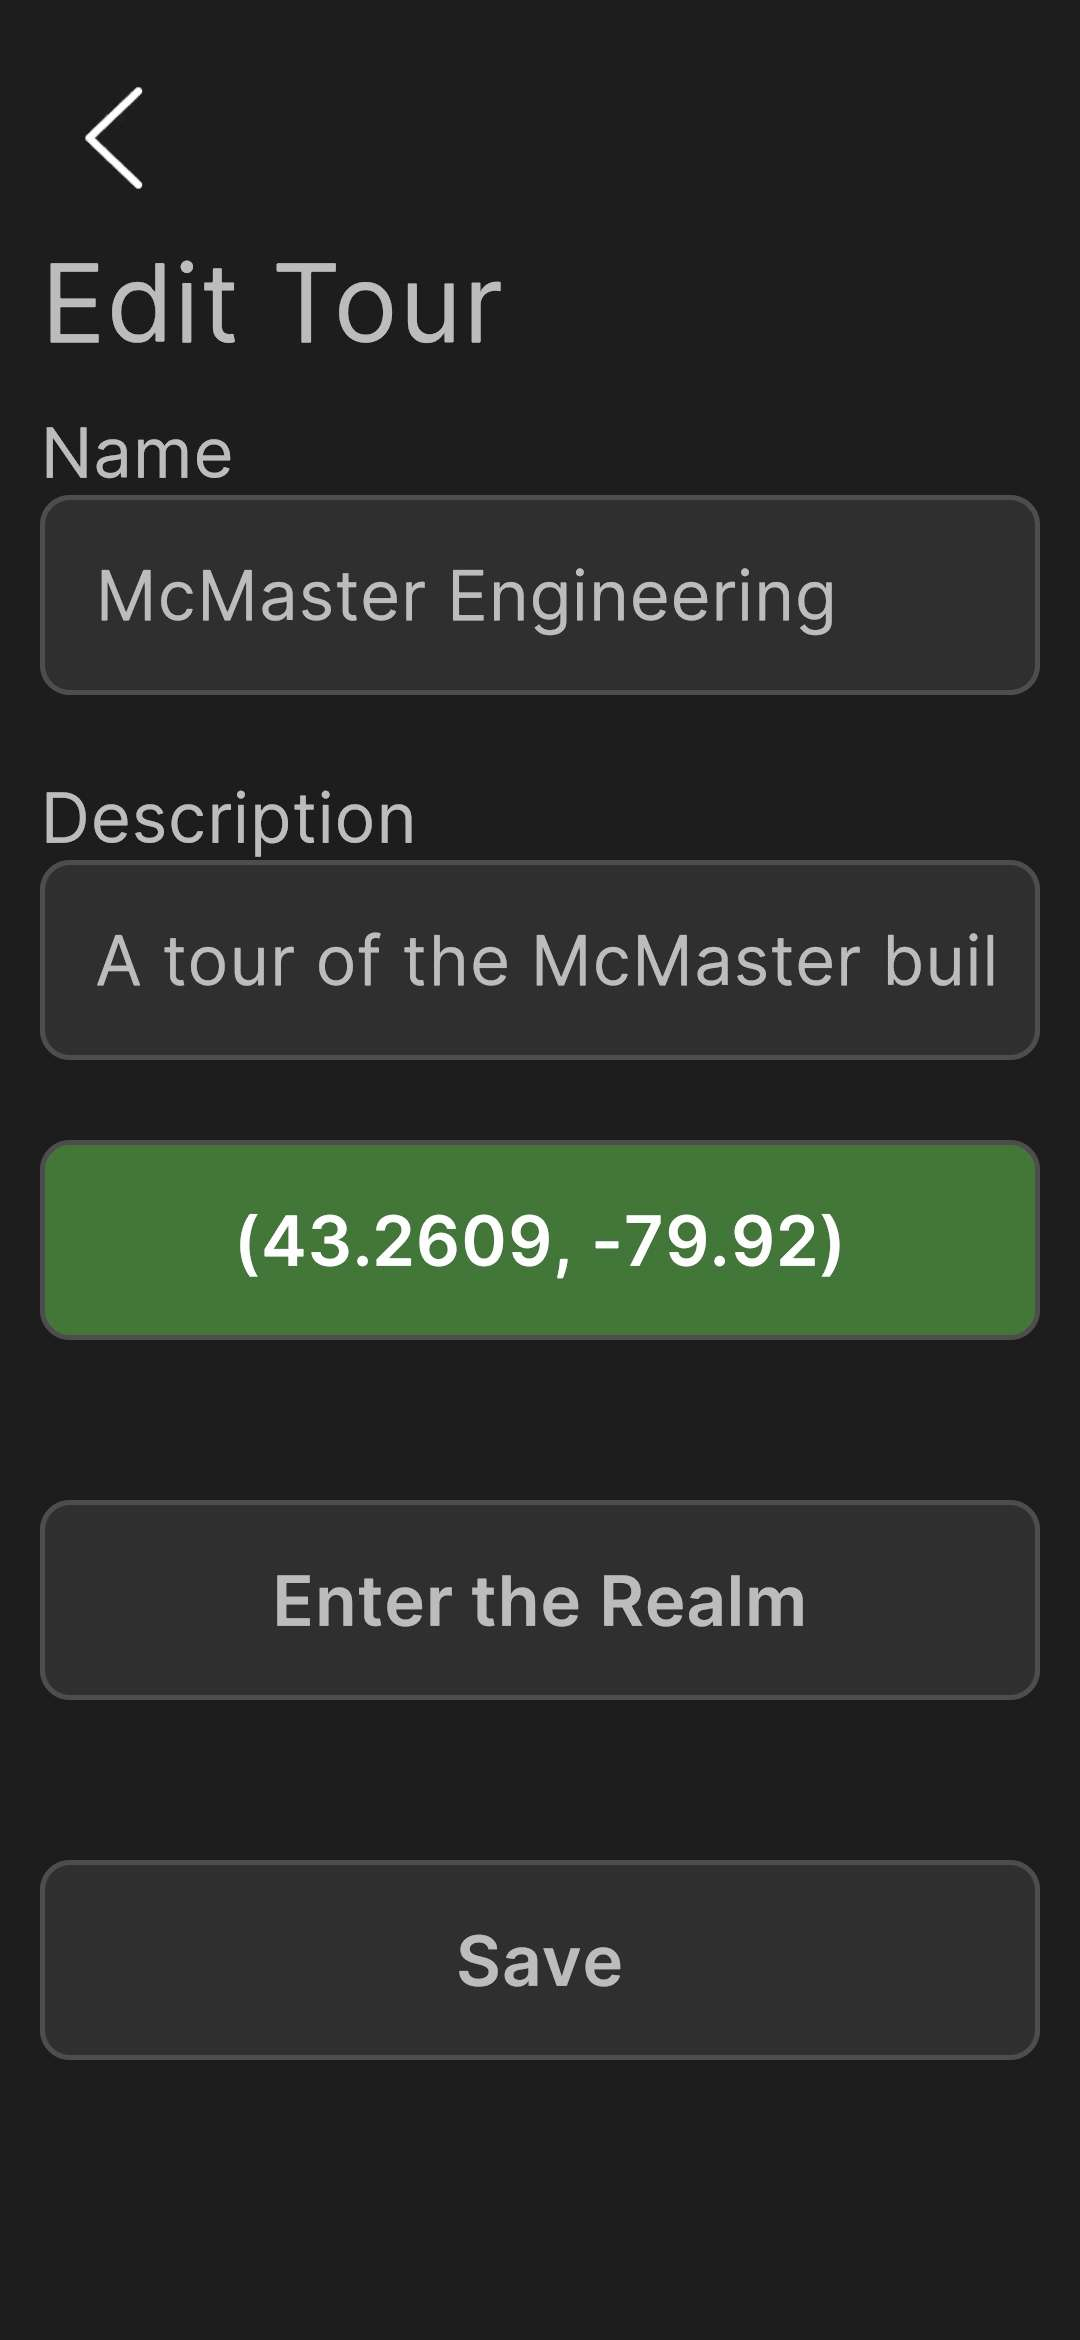
\includegraphics[width=\textwidth]{edit_tour.png}
    \end{subfigure}
    \caption{Edit Existing Tour}
    \label{fig:edit_tour}
\end{figure}

\newpage
\begin{figure}[ht!]
    \centering
    \begin{subfigure}[b]{0.48\textwidth}
        \centering
        \includegraphics[width=\textwidth]{obj_place1.png}
    \end{subfigure}
    \hfill
    \begin{subfigure}[b]{0.48\textwidth}
        \centering
        \includegraphics[width=\textwidth]{obj_place2.png}
    \end{subfigure}
    \caption{Object Placement in \progname{}}
    \label{fig:obj_place}
\end{figure}

\clearpage
\subsection{Viewing Tours on the Map}
\textbf{Overview:} The map feature offers an intuitive way to explore the geographical placement of AR tours and object clusters, helping users plan their navigation and discover nearby AR content.

\textbf{Key Features:}
\begin{itemize}[leftmargin=*]
    \item \textbf{Current Location:} Displays the user's current position along with nearby tours and AR objects.
    \item \textbf{Interactive Markers:} Markers indicate tour locations and can be selected to view detailed tour information.
    \item \textbf{Navigation Assistance:} Users can select markers to receive directions to a specific tour.
    \item \textbf{Restricted Areas:} The map identifies restricted zones and prevents navigation through these areas.
\end{itemize}

\textbf{How to Use:}
\begin{enumerate}[leftmargin=*]
    \item Open the \emph{Map} view from the \hyperref[fig:nav_bar]{navigation bar}.
    \item Zoom and pan around to see different tour markers.
    \item Tap a marker to view detailed information about the tour.
\end{enumerate}

\subsection{Generating a Custom AR Object via Prompt}
\textbf{Overview:} This functionality allows users to generate unique AR objects by entering a text prompt. The system processes the input, validates it, and produces an AR object that the user can preview and select.

\textbf{Key Features:}
\begin{itemize}[leftmargin=*]
    \item \textbf{Prompt Entry:} Users can enter a descriptive text prompt to define the desired AR object.
    \item \textbf{Object Generation:} The system generates an AR object based on the entered prompt.
    \item \textbf{Preview and Selection:} Users can rotate and preview the generated object, then choose to add it to their inventory.
\end{itemize}

\textbf{How to Use:}
\begin{enumerate}[leftmargin=*]
    \item From the Realm Interface, select the option to generate an AR object via prompt.
    \item Add a name for the object that is generated.
    \item Enter your descriptive prompt in the provided text field.
    \item Press ``Generate'' and submit the prompt.
    \item User must wait for around 1 minute for the object to be generated.
    \item Once generated, select the object to preview it in detail and add it to your inventory.
\end{enumerate}

\newpage
\begin{figure}[ht!]
    \setlength{\fboxrule}{0.1mm}
    \centering
    \begin{subfigure}[b]{0.48\textwidth}
        \centering
        \fbox{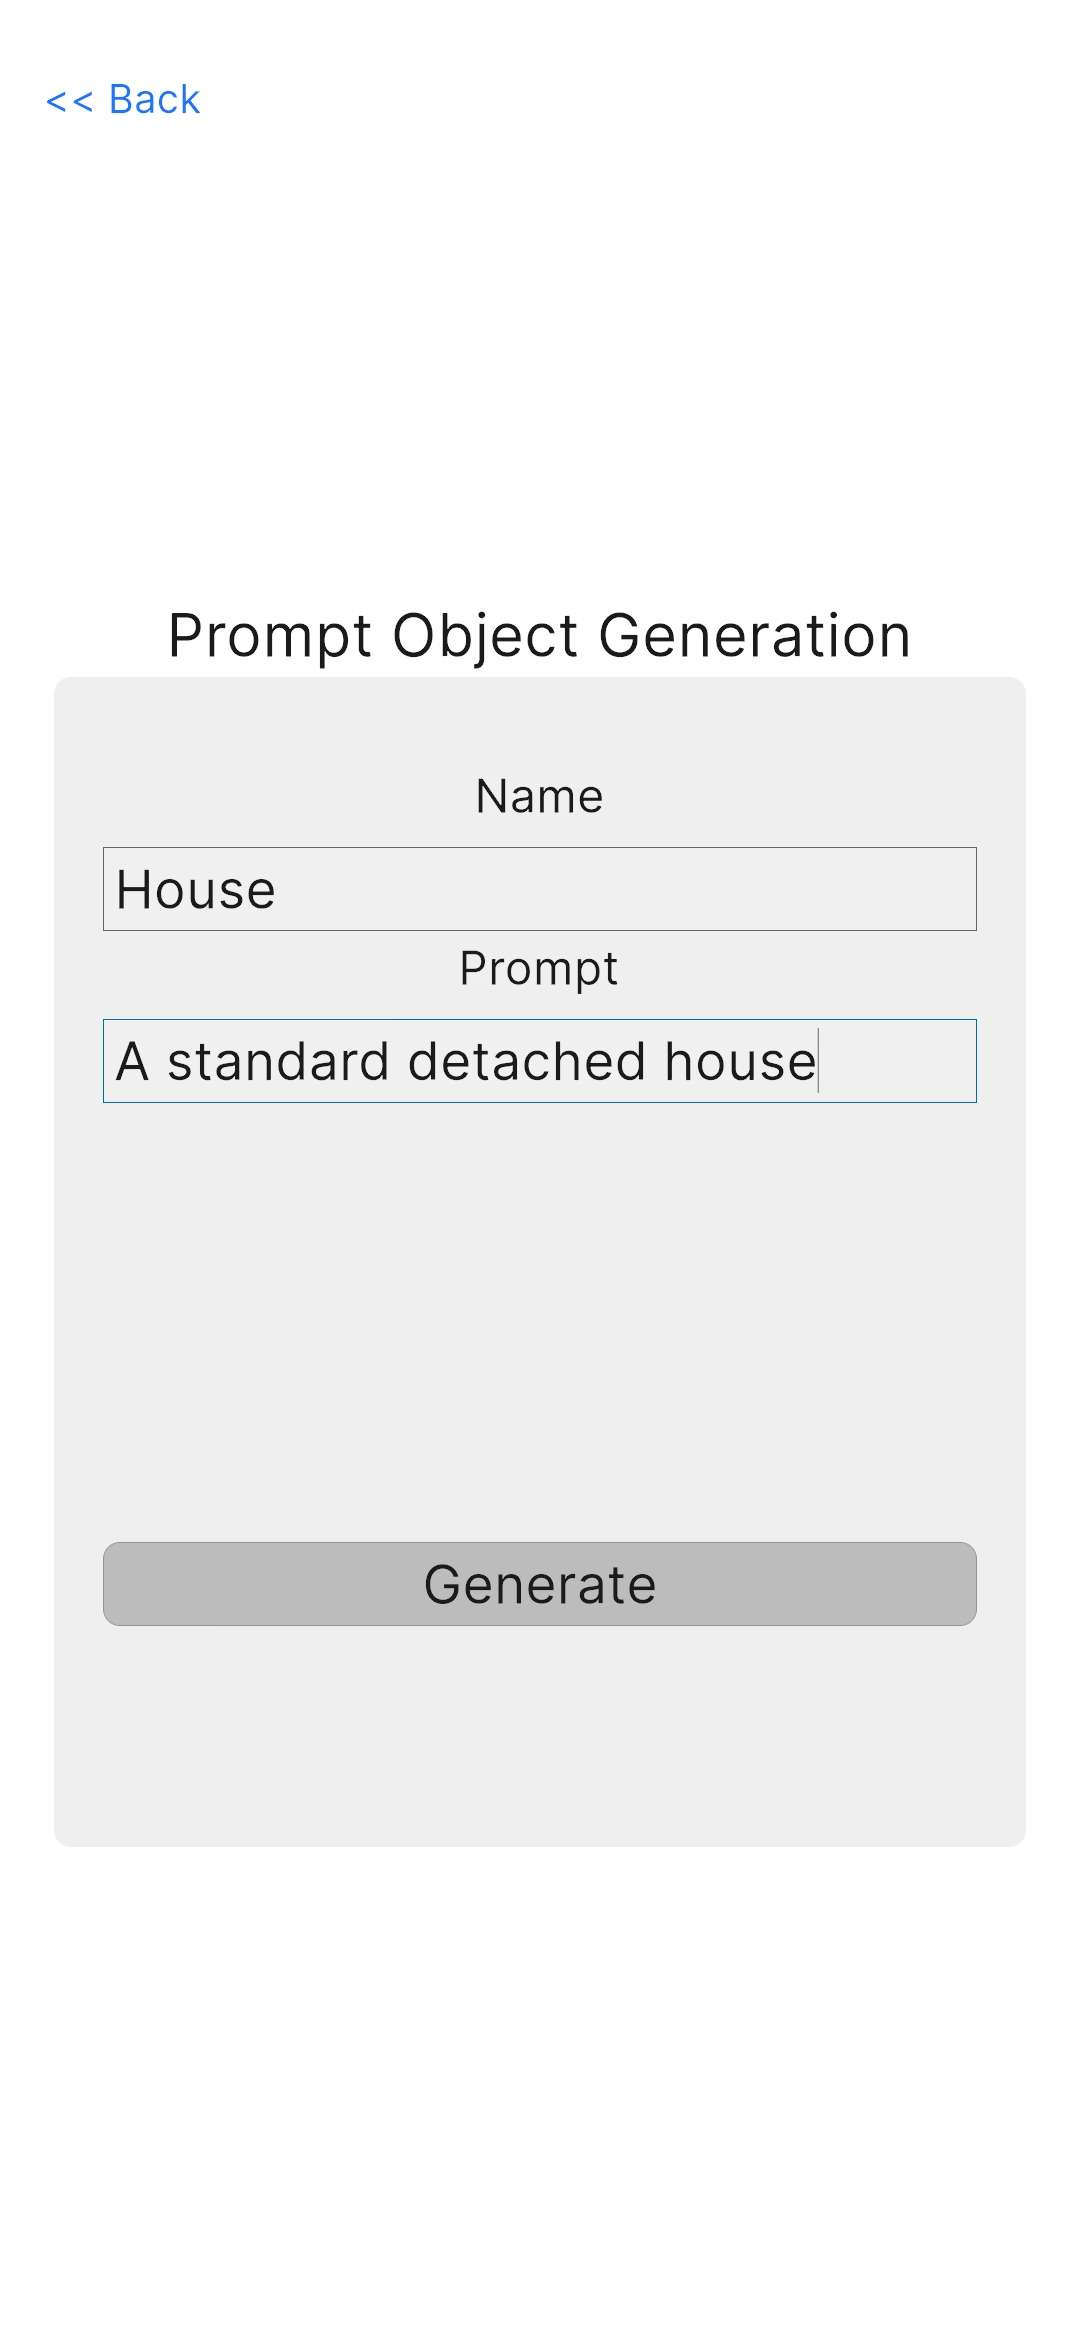
\includegraphics[width=\textwidth]{obj_gen1.png}}
    \end{subfigure}
    \hfill
    \begin{subfigure}[b]{0.48\textwidth}
        \centering
        \fbox{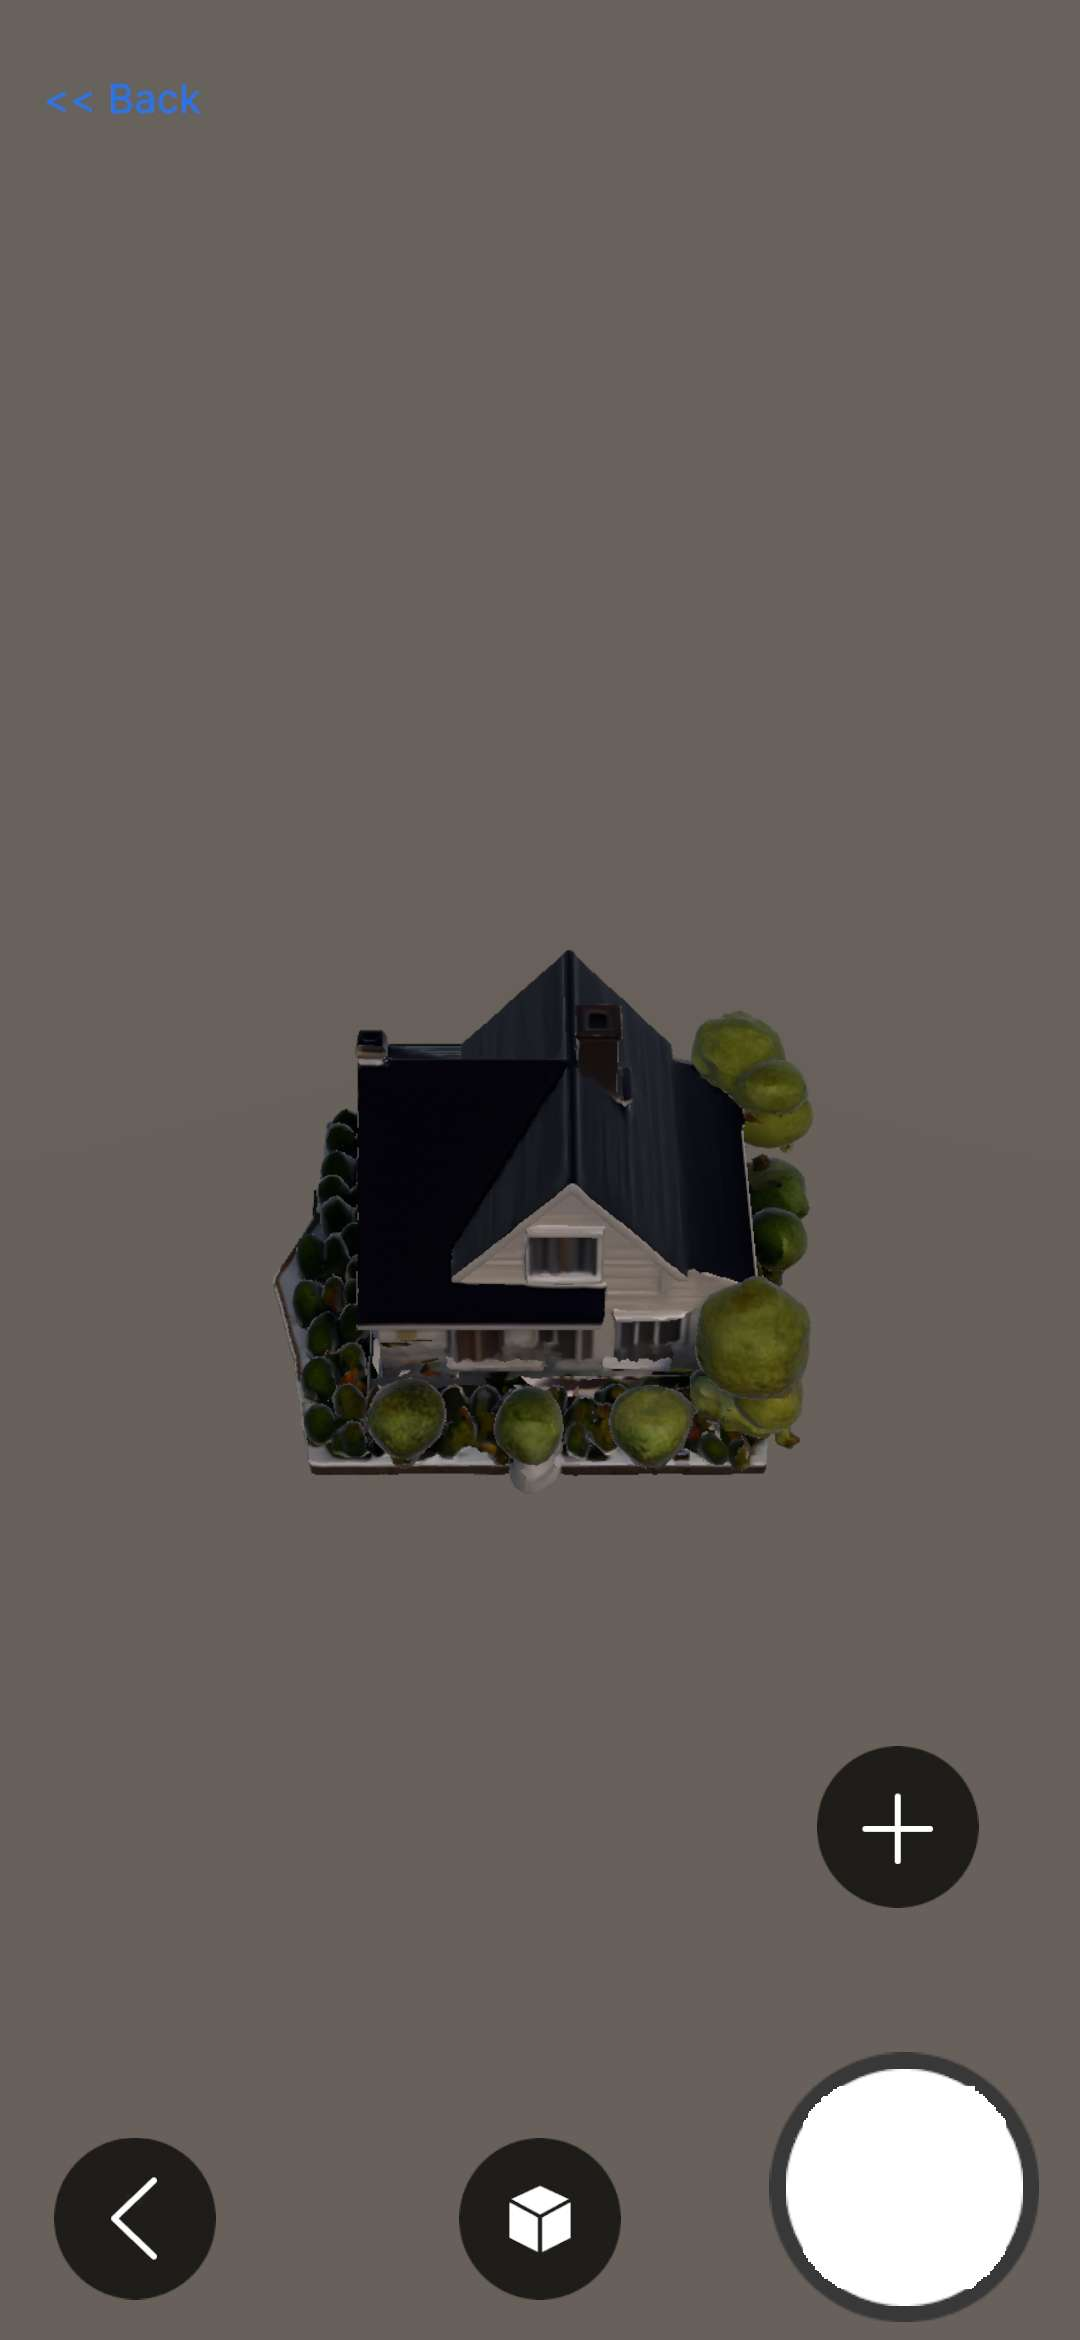
\includegraphics[width=\textwidth]{obj_gen2.png}}
    \end{subfigure}
    \caption{Prompt Object Generation in \progname{}}
    \label{fig:obj_gen}
\end{figure}

\newpage
\subsection{Profile Settings}
\textbf{Overview:} The Profile Screen is where users manage their account settings. It supports authentication and personal data management, allowing users to review and update their profile details.

\textbf{Key Features:}
\begin{itemize}[leftmargin=*]
    \item \textbf{Authentication:} Users enter valid credentials (username, email account and password) to log in.
    \item \textbf{Profile Information:} Users can view and update personal details such as their username and status, as well as change their password.
\end{itemize}

\textbf{How to Use:}
\begin{enumerate}[leftmargin=*]
    \item Log in to the app using your credentials.
    \item Navigate to the Profile section from the main Tours screen and select \emph{Profile Settings}.
    \item Edit the provided fields (e.g., username and password) and save your changes.
\end{enumerate}

\begin{figure}[ht!]
    \centering
    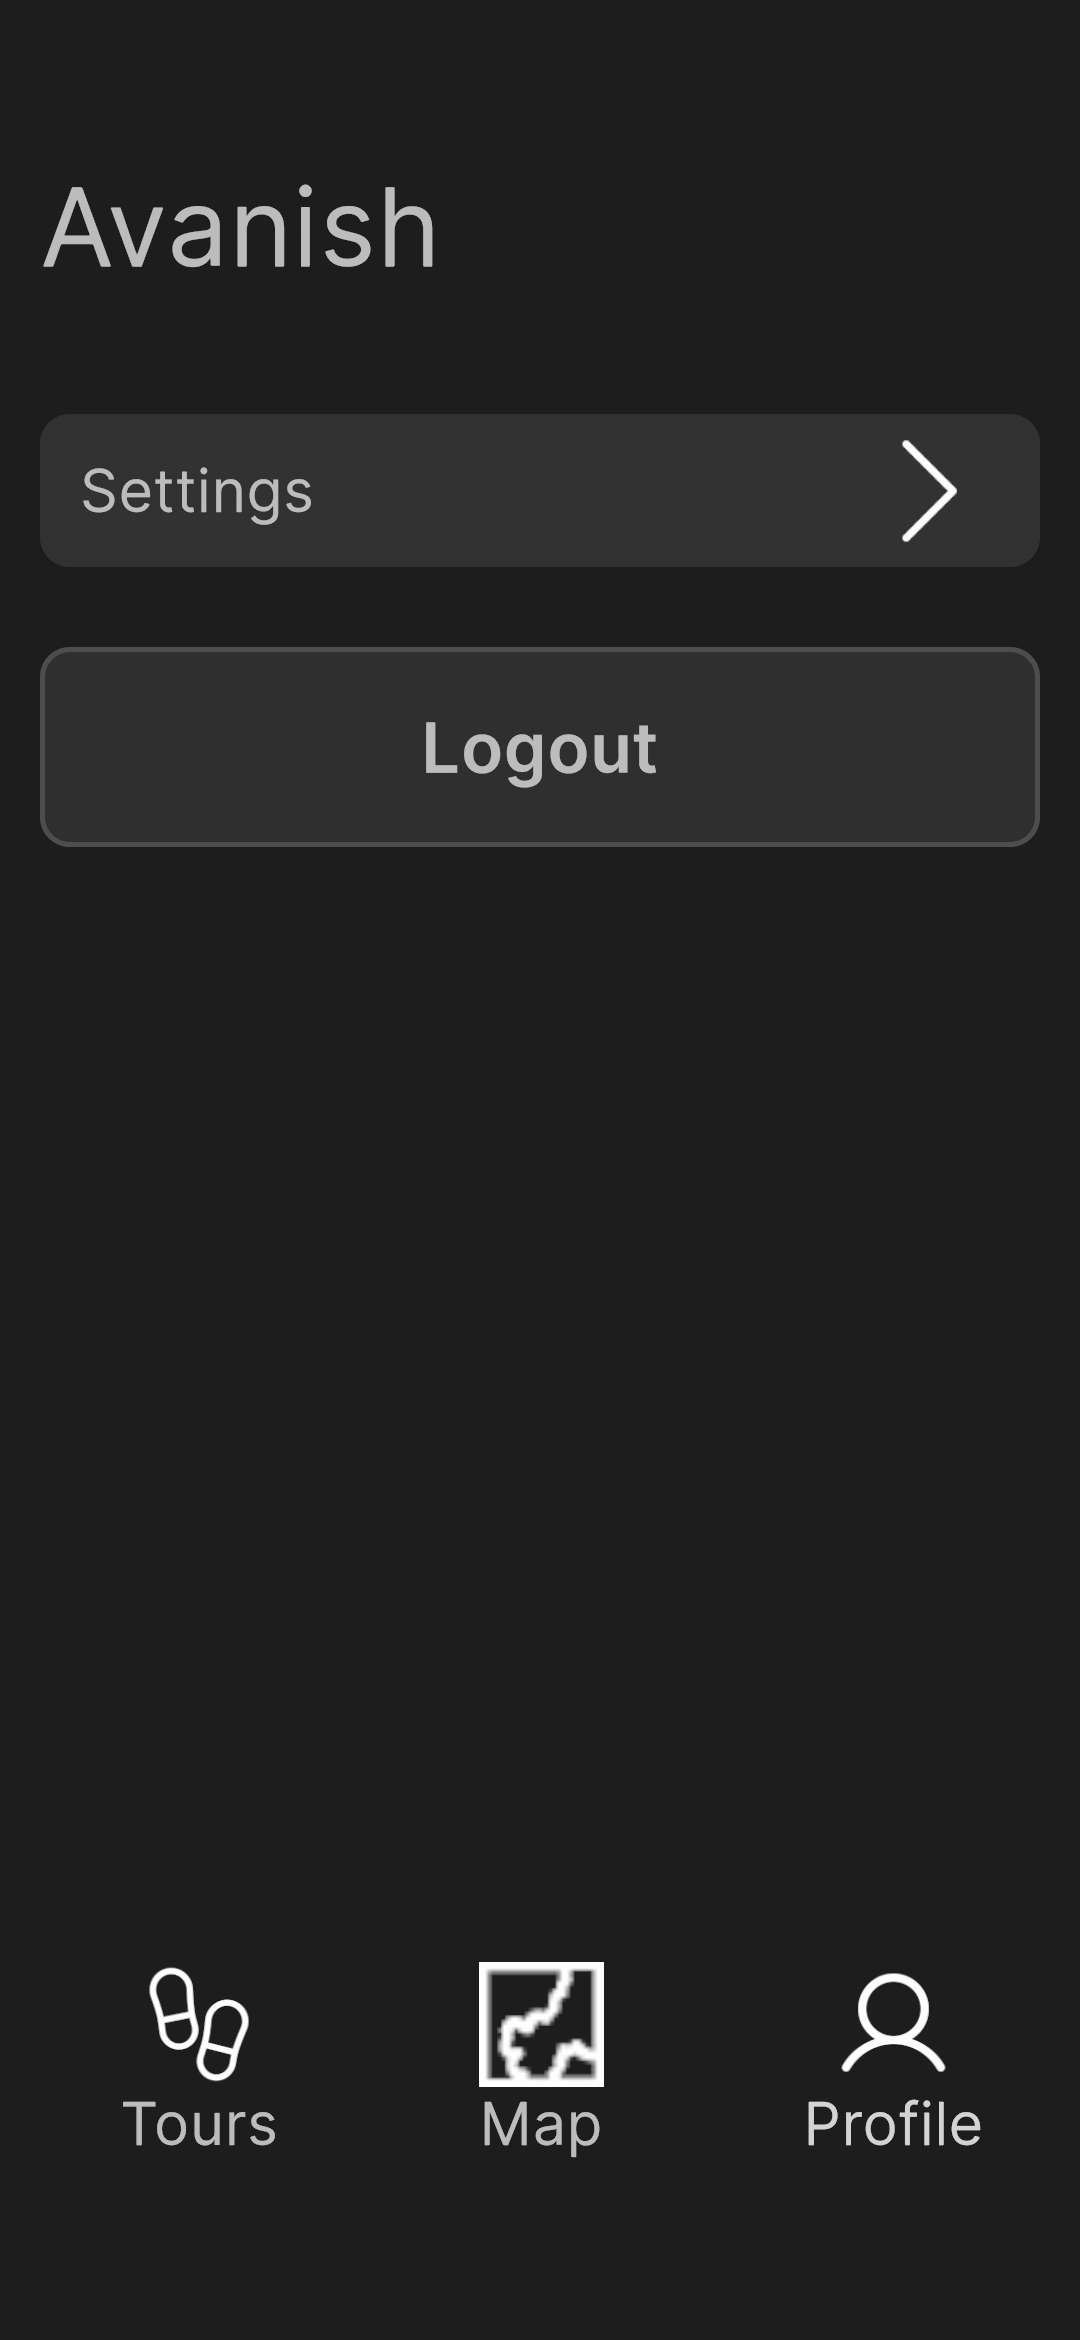
\includegraphics[width=0.33\textwidth]{profile.png}
    \caption{Profile Screen of \progname{}}
    \label{fig:profile}
\end{figure}
\clearpage

%-----------------------------

\newpage
\section{Appendix}

\subsection{Legal and Safety Information}
Include any legal disclaimers, copyright notices, or warranty information.
The application follows the \texttt{Apache License Version 2.0}. You can find a copy of the license, and its permissions and limitations in the app repository \href{https://github.com/russellrd/realm/blob/main/LICENSE}{here}.

%-----------------------------
\section{Feedback and Contact Information}

To provide user feedback, users can fill out the feedback survey form available \href{https://docs.google.com/forms/d/1vMPKYSl9AzGX9eO3fxNMUmQk0IhUB8fbnOACOne6x5Y/edit}{here}. Additionally, users can report bugs or issues directly to the developer team via email.

\end{document}
